  \documentclass[14pt, oneside]{book}
    \usepackage[margin=1in]{geometry} 
    \usepackage[brazilian]{babel}
    \usepackage{graphicx}
    \usepackage[utf8]{inputenc}
    \usepackage[T1]{fontenc}
    \usepackage{amsmath,amsthm,amssymb,amsfonts, mathtools}
    \usepackage{enumitem, verbatim, tikz, multicol}
    \usepackage{titlesec,hyperref, color, float, comment}
    
        \hypersetup{
            colorlinks=false, %set true if you want colored links
            linktoc=all,     %set to all if you want both sections and subsections linked
            linkcolor=blue,  %choose some color if you want links to stand out
        }
    \usepackage{listings}
    \titleformat{\chapter}[hang]{\bf\huge}{\thechapter}{2pc}{}
    \DeclarePairedDelimiter{\ceil}{\lceil}{\rceil}
    \date{\vspace{-5ex}}
    \lstset{language=Python}  
    \usepackage{pythonhighlight}
     
    \newcommand{\N}{\mathbb{N}}
    \newcommand{\Z}{\mathbb{Z}}
    \newcommand\tab[1][1cm]{\hspace*{#1}}
    \renewcommand{\qedsymbol}{$\blacksquare$}
     
    
\theoremstyle{definition}
    \newtheorem{problem}{Problema}
    \newtheorem{dica}{Dica}
    \newtheorem{gabarito}{Gabarito}
    \newtheorem{defn}{Definição}
    \newtheorem{teorema}{Teorema}
    
\begin{document}
    \pagenumbering{gobble}

    \begin{titlepage}
        \centering 
        
\includegraphics[scale = 0.8]{ufpe.png} \\
        \Large{\textbf{UNIVERSIDADE FEDERAL DE PERNAMBUCO}}\\
        \large{Departamento de Eletrônica e Sistemas}
        \vspace*{\stretch{2.0}}
   
        \Huge\textbf{ELETRÔNICA DIGITAL}\\
        \Large\textbf{JOGO DE REPETIÇÃO}
   
        \vspace*{\stretch{2.0}}
        \vfill
        \Large{Arthur Santos Pimentel} \\
        \Large{Matheus Henrique Camilo de Araújo} \\
        \Large{Matheus Sobreira Farias} \\
        \Large{Pablo Godoy de Albuquerque}
        \\~\\
        \Large{Novembro, 2018}
    \end{titlepage}

\addtocontents{toc}{\protect\hypertarget{toc}{}}
\tableofcontents
\mainmatter
        \chapter[Motivação]{\hyperlink{toc}{Motivação}}
            \tab Como explicado no projeto anterior, existem linguagens de descrição de Hardware que podem descrever o funcionamento de um circuito e, portanto facilitar o trabalho do projetista ao sintetizar seu projeto em forma de circuito. Neste projeto, com o auxílio da linguagem de descrição VHDL, pode-se observar o avanço devido às ferramentas disponibilizadas por uma linguagem. A grande economia de tempo acarreta na produtividade e agilidade da implementação de um projeto. Por exemplo, quando a linguagem de blocos no primeiro projeto foi usada, os grupos levaram em média duas semanas e meia para atingir as especificações do projeto. Agora, porém, com o auxílio de uma linguagem de descrição, nota-se que vários grupos concluiram o projeto mais cedo e tiveram tempo para debater as soluções de certos bugs. \\
	        \tab Ainda pode-se dizer que o uso de uma linguagem possibilitou a discussão sobre certos pontos do projeto entre integrantes do grupo, já que a descrição dos circuitos se tornou um processo menos mecânico. Quando os integrantes do grupo se dividiam em tarefas, geralmente, as ideias surgiam e os circuitos eram manualmente implementados no \textit{Quartus}. Agora, porém, os circuitos são interpretados pelo programa através de uma linguagem em códigos e transformadas nas versões mais simplistas de seus circuitos. Assim, o grupo se preocupa menos com a estética e a legibilidade do bloco e passa a focar em suas funcionalidades.\\
	        \tab HDLs podem descrever o funcionamento do circuito, a sua concepção e organização, e ainda testá-lo para verificar seu funcionamento por meio de simulação. São padrões de expressões baseados em texto, da estrutura espacial, temporal e comportamental dos sistemas eletrônicos. Como outras linguagens de programação, HDLs incluem anotações explícitas para expressar a simultaneidade bem como sintaxe e semântica próprias. No entanto, em contraste com a maioria dos softwares de linguagem de programação, HDLs também incluem uma noção implícita de tempo, como um atributo primário de hardware. \\
	        \tab A linguagem VHDL foi desenvolvida, em meados da década de 1980, para substituir os complexos manuais que descreviam o funcionamento dos 	ASICs. Como o próprio nome indica, VHDL significa linguagem de descrição de hardwares para circuitos integrados de altíssima velocidade. Ela pode descrever o comportamento e a estrutura de sistemas eletrônicos, mas é particularmente adequada como uma linguagem para descrever a estrutura e o 		comportamento de projetos de hardware, como ASICs e FPGAs, bem como circuitos digitais convencionais. Uma característica importante da linguagem VHDL é que ela é fortemente tipificada. \\
	        \tab Geralmente, uma linguagem fortemente tipada tem regras de digitação mais rígidas em tempo de compilação, o que implica que erros e exceções são mais prováveis de acontecer durante a compilação. A maioria dessas regras afeta a atribuição de variáveis, os valores de retorno e a chamada de função. Essas linguagens são aquelas em que todas as variáveis tem um tipo específico e seus tipos são importantes para a linguagem. O que significa que uma vez que a variável foi declarada com um tipo ela será até o seu fim do mesmo tipo. Por outro lado, uma linguagem fracamente tipada possui regras de digitação mais flexíveis e pode produzir resultados imprevisíveis. "ou pode executar conversão de tipo implícita em tempo de execução."
	        
           
            
        \chapter[Objetivos]{\hypertarget{obj}{}\hyperlink{toc}{Objetivos}}
             \tab Nesse projeto, foi utilizada a linguagem de descrição de Hardware VHDL, com o auxílio do software \textit{Quartus Prime 17.1} e da placa \textit{FPGA DE2-155}, ambos da \textit{Altera}, com o intuito de criar um jogo de repetição, seguindo os seguintes critérios:
            \begin{itemize}
                \item Uma chave dá inicio ao jogo.
                \item Exibe-se a fase do jogo e em seguida exibe-se a sequência gerada aleatoriamente por um tempo dependente da fase.
                \item Pede-se para o jogador digitar no controle remoto a sequência mostrada anteriormente.
                \item Usa-se 8 LEDs para indicar o recebimento dos números enviados pelo controle.
                \item Caso o jogador acerte a sequência, o jogo passa para a próxima fase e o tempo de exibição da sequência diminui em 20\%.
                \item Caso o jogador erre a sequência, o jogo permanece na mesma fase e o jogador perde uma vida.
                \item Após 4 acertos o jogador vence o jogo.
                \item Após 3 erros o jogador perde o jogo.
                \item Por último, exibe-se os créditos com os nomes dos integrantes da equipe.
            \end{itemize}
            
            
        \chapter[Implementação]{\hyperlink{toc}{Implementação}}
            \tab Para realizar a implementação do jogo de repetição, foi utilizado o software \textit{Quartus Prime 17.1}, que é um software cuja função é ser um ambiente de desenvolvimento para linguagens de descrição de hardware, sendo assim, a placa a qual foi descrita pelo projeto foi a \textit{Altera DE2-115}. Foi utilizada ao longo do desenvolvimento a linguagem de descrição de hardware VHDL. \\
            \tab Uma vez no software \textit{Quartus}, para facilitar a construção do projeto, foi decidido separá-lo em \textbf{4} módulos de desenvolvimento, dessa forma o grupo como um todo conseguiria agir paralelamente, para que o tempo fosse melhor otimizado, são estes os módulos: \textbf {LCD}, \textbf{logica\_jogo}, \textbf{Infravermelho}, \textbf{Random}...
            
            \section[LCD]{\hyperlink{toc}{LCD}}
            \tab O módulo LCD da placa utilizada é de tamanho 16x2 e pode ser utilizado através de envio de comandos apropriados para aparecer o que se deseja na tela de video, o seu controlador se denomina $HD44780$. \\
            \tab Tal controlador pode enviar/receber dados em duas operações de 4 bits ou em uma operação de 8 bits. Para a interface de dados de 4 bits, somente quatro linhas de barramento DB4 a DB7 são usadas para transferência. As linhas de barramento DB0 a DB3 são desativadas. \\
            \tab A transferência de dados entre o $HD44780$ e a $FPGA$ é concluida após os dados de 4 bits terem sido transferidos duas vezes. Quanto à ordem de transferência de dados, os quatro obits mais significativos são transferidos antes dos quatro bits menos significativos. \\
            \tab Para interface de dados de 8 bits, todas as oito linhas de barramento (DB0 a DB7) são usadas.
            \tab Para poder imprimir na tela o coração, foi preciso utilizar um espaço vazio do CGRAM e preenche-lo da forma apropriada, atribuindo valor logico alto para o quadrado corresponde ficar pintado escuro, e atribuindo valor logico baixo para o quadrado corresponder ficar claro, e assim poder ser feito o desenho do coração. As Figuras abaixo mostram peças importantes no estudo do LCD, desde seu esquemático até as figuras pre-estabelecidas do CGRAM.
                \begin{figure}[H]
                    \centering
                    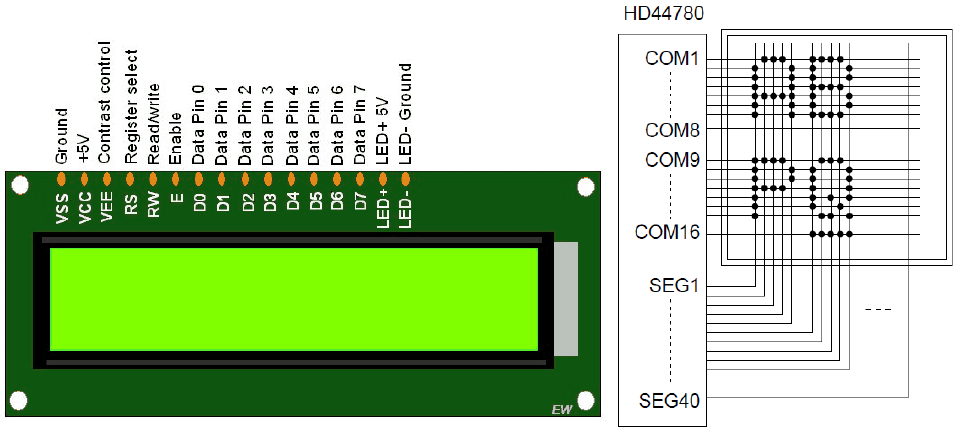
\includegraphics[scale=0.8]{lcd1.png}
                    \caption{Caracterização do LCD}
                    \label{lcd1}
                \end{figure}\\
                
                \begin{figure}[H]
                    \centering
                    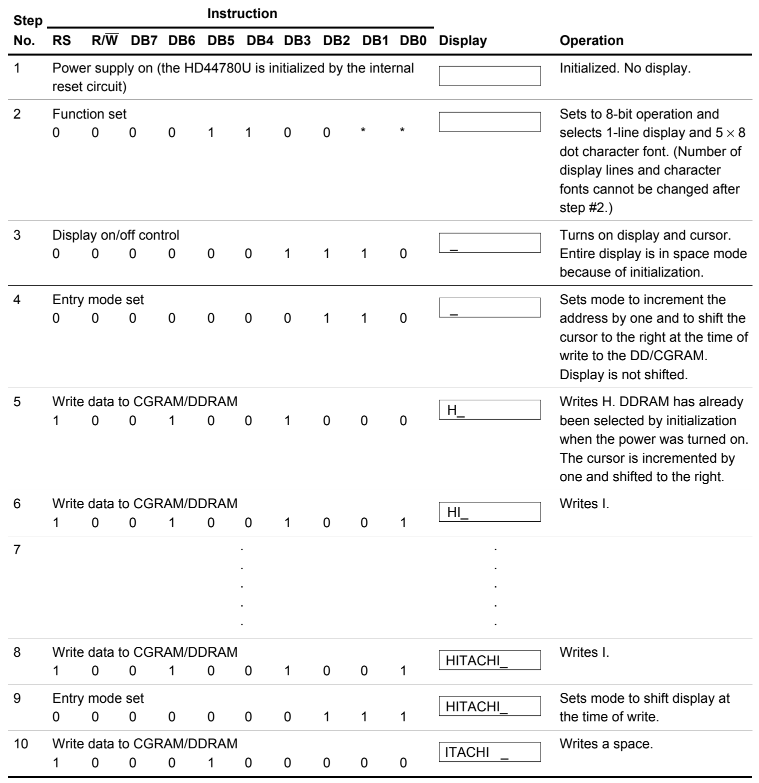
\includegraphics[scale=1]{lcd2.png}
                    \caption{Datasheet - Comandos de uso do LCD 1}
                    \label{lcd2}
                \end{figure} \\
                
                \begin{figure}[H]
                    \centering
                    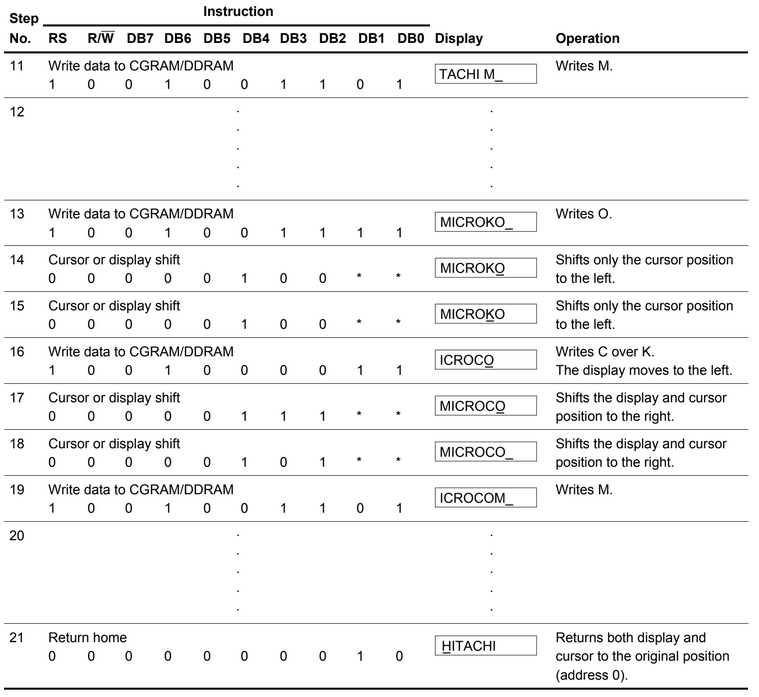
\includegraphics[scale=1]{lcd3.png}
                    \caption{Datasheet - Comandos de uso do LCD 2}
                    \label{lcd3}
                \end{figure} \\
                
                \begin{figure}[H]
                    \centering
                    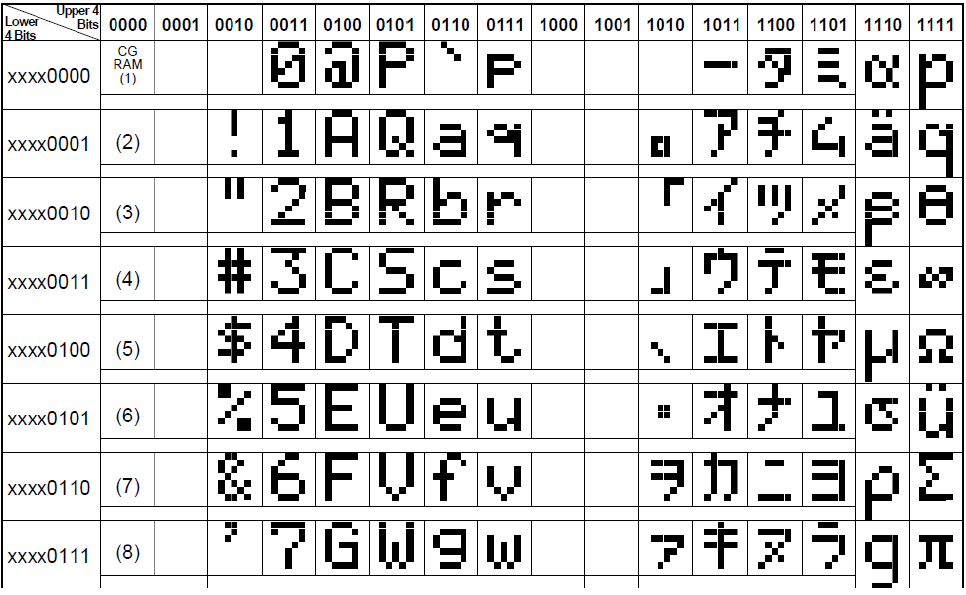
\includegraphics[scale=0.8]{lcd4.png}
                    \caption{Datasheet - Figuras do CGRAM 1}
                    \label{lcd4}
                \end{figure} \\
                
                \begin{figure}[H]
                    \centering
                    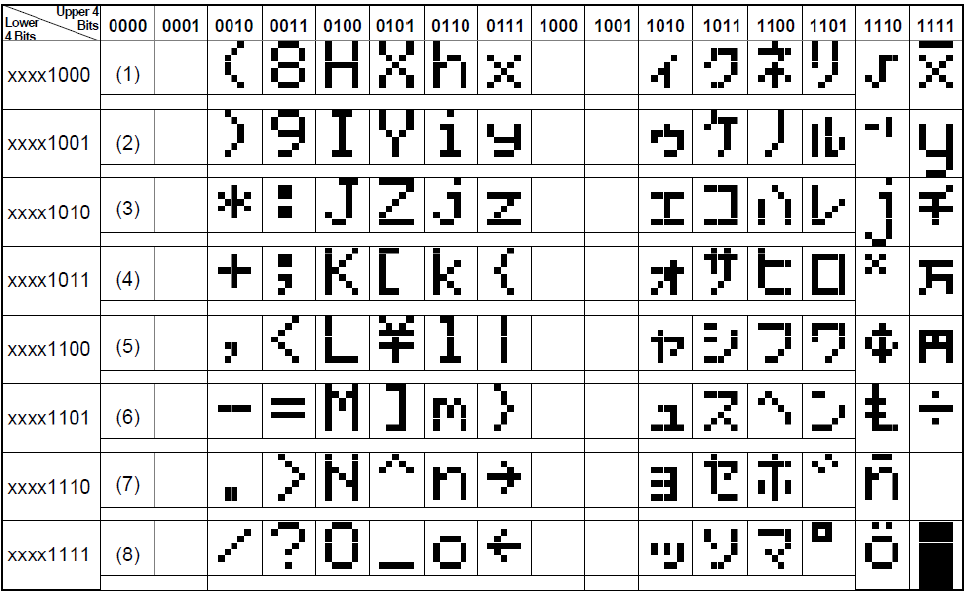
\includegraphics[scale=0.8]{lcd5.png}
                    \caption{Datasheet - Figuras do CGRAM 2}
                    \label{lcd5}
                \end{figure}
                
                
                \subsection[lcd\_example]{\hyperlink{toc}{lcd\_example}}
                \tab É parte do código relacionada à utilização do LCD, inserindo os textos correspondentes a cada estado da máquina. Segue as Figuras abaixo que representam o código relacionado a cada estado.
                
                \begin{figure}[H]
                    \centering
                    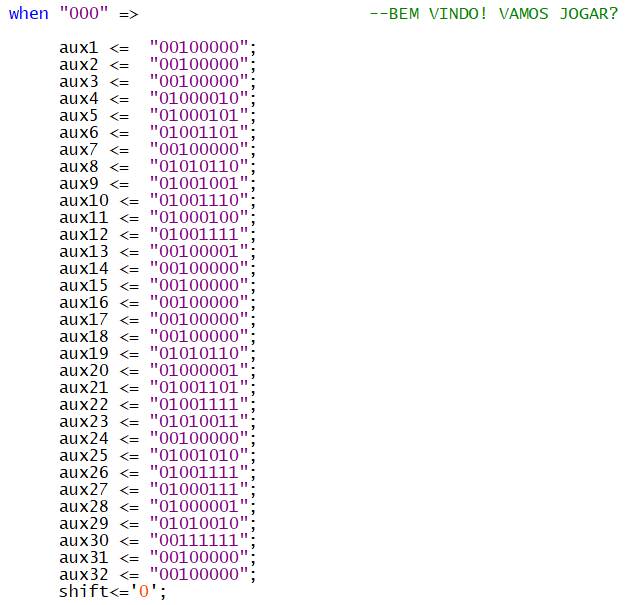
\includegraphics[scale=1]{lcdexample1.png}
                    \caption{BEM VINDO! VAMOS JOGAR?}
                    \label{lcdexample1}
                \end{figure}
                
                \begin{figure}[H]
                    \centering
                    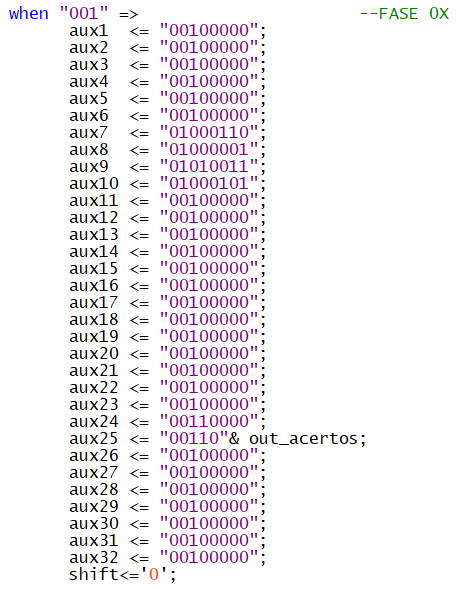
\includegraphics[scale=1]{lcdexample2.png}
                    \caption{FASE 0X}
                    \label{lcdexample2}
                \end{figure}
                
                \begin{figure}[H]
                    \centering
                    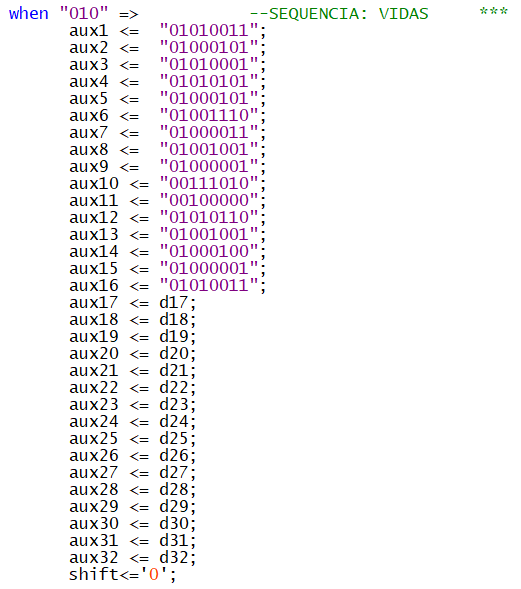
\includegraphics[scale=1]{lcdexample3.png}
                    \caption{SEQUÊNCIA: VIDAS}
                    \label{lcdexample3}
                \end{figure}
                
                \begin{figure}[H]
                    \centering
                    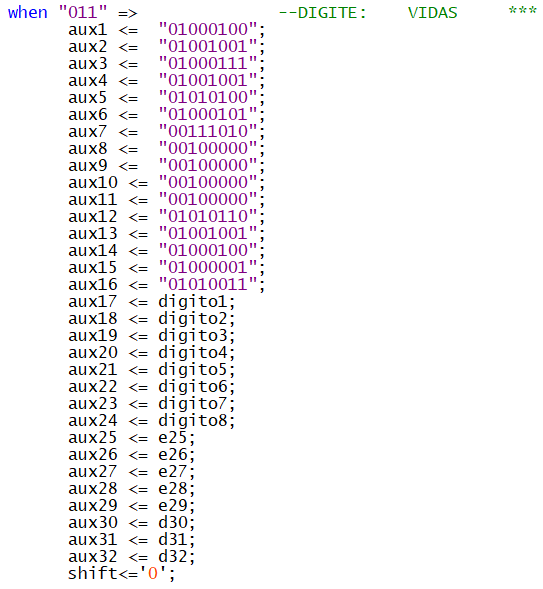
\includegraphics[scale=1]{lcdexample4.png}
                    \caption{DIGITE: VIDAS}
                    \label{lcdexample4}
                \end{figure}
                
                \begin{figure}[H]
                    \centering
                    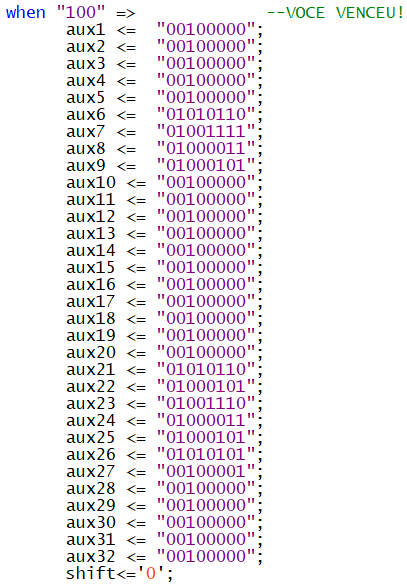
\includegraphics[scale=1]{lcdexample5.png}
                    \caption{VOCÊ VENCEU!}
                    \label{lcdexample5}
                \end{figure}
                
                \begin{figure}[H]
                    \centering
                    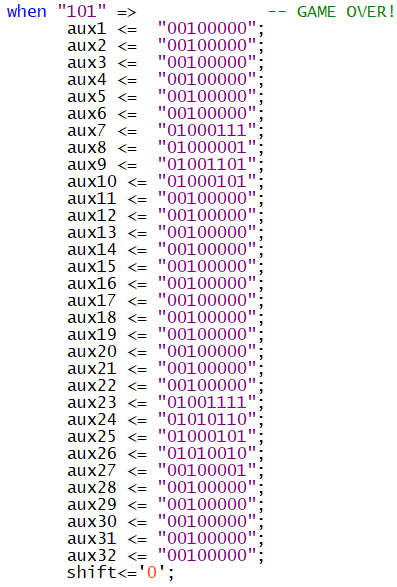
\includegraphics[scale=1]{lcdexample6.png}
                    \caption{GAME OVER!}
                    \label{lcdexample6}
                \end{figure}
                
                \begin{figure}[H]
                    \centering
                    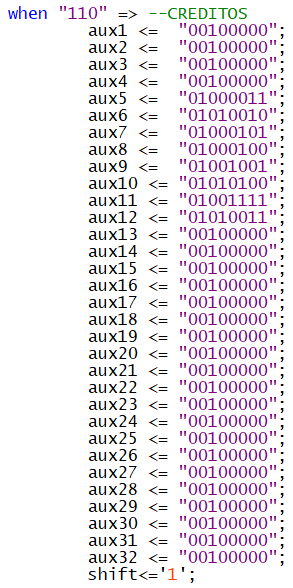
\includegraphics[scale=1]{lcdexample7.png}
                    \caption{CREDITOS}
                    \label{lcdexample7}
                \end{figure}
                
                \subsection[lcd\_controller]{\hyperlink{toc}{lcd\_controller}}
                \tab Como o próprio nome sugere, este módulo atua como o controlador das operações do LCD, para não ter que elaborá-lo desde o inicio, este código foi copiado da internet, entendido e aí sim foi possível fazer equivalências para que funcionasse perfeitamente com o projeto todo. Segue na Figura \ref{lcdcontroller} um pequeno trecho do código.
                
                \begin{figure}[H]
                    \centering
                    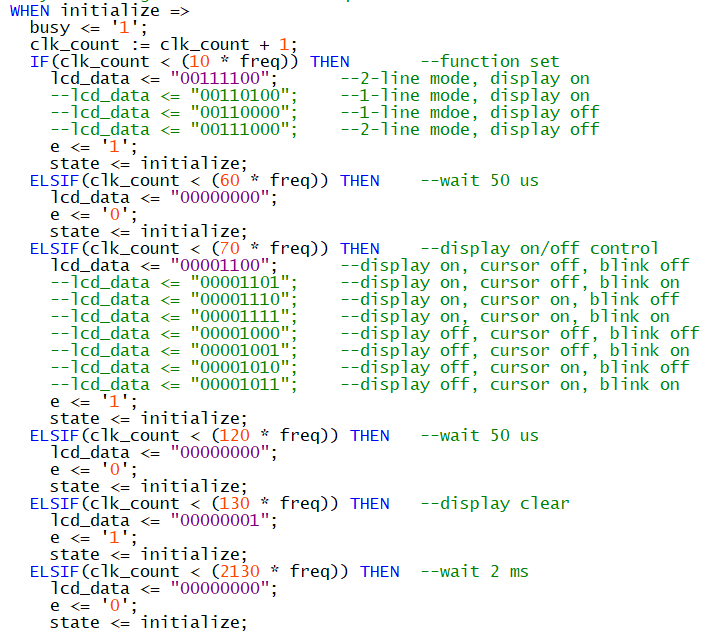
\includegraphics[scale=1]{lcdcontroller.png}
                    \caption{Código do LCD Controller}
                    \label{lcdcontroller}
                \end{figure}
               
                
            \section[logica\_jogo]{\hyperlink{toc}{logica\_jogo}}
            
               \tab A lógica do jogo foi implementada usando Máquinas de Estados Finitos. A representação da lógica do jogo por uma Maquina de Estados é vista a seguir:
                \begin{center}
                    \begin{tikzpicture}[scale=0.2]
                        \tikzstyle{every node}+=[inner sep=0pt]
                        \draw [black] (38.4,-4.6) circle (3);
                        \draw (38.4,-4.6) node {$S_0$};
                        \draw [black] (38.4,-15.5) circle (3);
                        \draw (38.4,-15.5) node {$S_1$};
                        \draw [black] (38.4,-26.5) circle (3);
                        \draw (38.4,-26.5) node {$S_2$};
                        \draw [black] (53.6,-45.4) circle (3);
                        \draw (53.6,-45.4) node {$S_5$};
                        \draw [black] (23.6,-45.4) circle (3);
                        \draw (23.6,-45.4) node {$S_4$};
                        \draw [black] (38.4,-56.4) circle (3);
                        \draw (38.4,-56.4) node {$S_6$};
                        \draw [black] (38.4,-38.1) circle (3);
                        \draw (38.4,-38.1) node {$S_3$};
                        \draw [black] (38.4,-7.6) -- (38.4,-12.5);
                        \fill [black] (38.4,-12.5) -- (38.9,-11.7) -- (37.9,-11.7);
                        \draw (37.9,-10.05) node [left] {$chave\mbox{ }=\mbox{ }'1'$};
                        \draw [black] (38.4,-18.5) -- (38.4,-23.5);
                        \fill [black] (38.4,-23.5) -- (38.9,-22.7) -- (37.9,-22.7);
                        \draw (37.9,-21) node [left] {$5\mbox{ }segundos$};
                        \draw [black] (26.01,-47.19) -- (35.99,-54.61);
                        \fill [black] (35.99,-54.61) -- (35.65,-53.73) -- (35.05,-54.53);
                        \draw (26.02,-51.4) node [below] {$5\mbox{ }segundos$};
                        \draw [black] (51.17,-47.16) -- (40.83,-54.64);
                        \fill [black] (40.83,-54.64) -- (41.77,-54.58) -- (41.19,-53.77);
                        \draw (50.97,-51.4) node [below] {$5\mbox{ }segundos$};
                        \draw [black] (35.417,-4.785) arc (301.27916:13.27916:2.25);
                        \draw (31.44,-1.06) node [left] {$chave\mbox{ }=\mbox{ }'0'$};
                        \fill [black] (36.44,-2.35) -- (36.45,-1.4) -- (35.6,-1.92);
                        \draw [black] (38.4,-29.5) -- (38.4,-35.1);
                        \fill [black] (38.4,-35.1) -- (38.9,-34.3) -- (37.9,-34.3);
                        \draw (38.9,-32.3) node [right] {$tempo\mbox{ }variavel$};
                        \draw [black] (35.44,-38.534) arc (-88.9849:-271.0151:11.736);
                        \fill [black] (35.44,-15.07) -- (34.65,-14.55) -- (34.63,-15.55);
                        \draw (23,-26.8) node [left] {$igual\mbox{ }='0'$};
                        \draw [black] (41.377,-15.207) arc (88.21798:-88.21798:11.599);
                        \fill [black] (41.38,-15.21) -- (42.16,-15.73) -- (42.19,-14.73);
                        \draw (53.12,-26.8) node [right] {$igual\mbox{ }='1'$};
                        \draw [black] (35.71,-39.43) -- (26.29,-44.07);
                        \fill [black] (26.29,-44.07) -- (27.23,-44.17) -- (26.79,-43.27);
                        \draw (26.98,-41.23) node [above] {$certo\mbox{ }=\mbox{ }4$};
                        \draw [black] (41.1,-39.4) -- (50.9,-44.1);
                        \fill [black] (50.9,-44.1) -- (50.39,-43.3) -- (49.96,-44.21);
                        \draw (57.55,-41.18) node [above] {$erros\mbox{ }=\mbox{ }3\mbox{ }ou\mbox{ }Tempo\mbox{ }>\mbox{ }1\mbox{ }min$};
                    \end{tikzpicture}
                \end{center}
                \tab Cada estado está associado a uma mensagem exibida pelo LCD. Estes são:        
                \begin{itemize}
                    \item $S_0$ corresponde a mensagem: BEM VINDO! VAMOS JOGAR?
                    \item $S_1$ corresponde a mensagem: FASE 0X.
                    \item $S_2$ corresponde a mensagem: SEQUÊNCIA. 
                    \item $S_3$ corresponde a mensagem: DIGITE. 
                    \item $S_4$ corresponde a mensagem: VOCÊ VENCEU!
                    \item $S_5$ corresponde a mensagem: GAME OVER!
                    \item $S_6$ corresponde a mensagem: TUCA FAFA PABLITO TETEU (CREDITOS).
                \end {itemize}
                \tab Nota-se que, no estado $S_3$, \textit{igual} $=$ '$1$' e \textit{igual} $=$ '$0$' possuem o mesmo destino. No entanto, dependendo do camiho percorrido, as variáveis \textit{acertos}, \textit{erros} e \textit{vidas} possuirão diferentes valores. Essa lógica pode ser vista nas linhas $146$ a $165$ do código da lógica do jogo. \\
                \tab Mostra-se a principal parte do código nas Figuras \ref{parte1} e \ref{parte2}.
                    
               \begin{figure}[H]
                    \centering
                    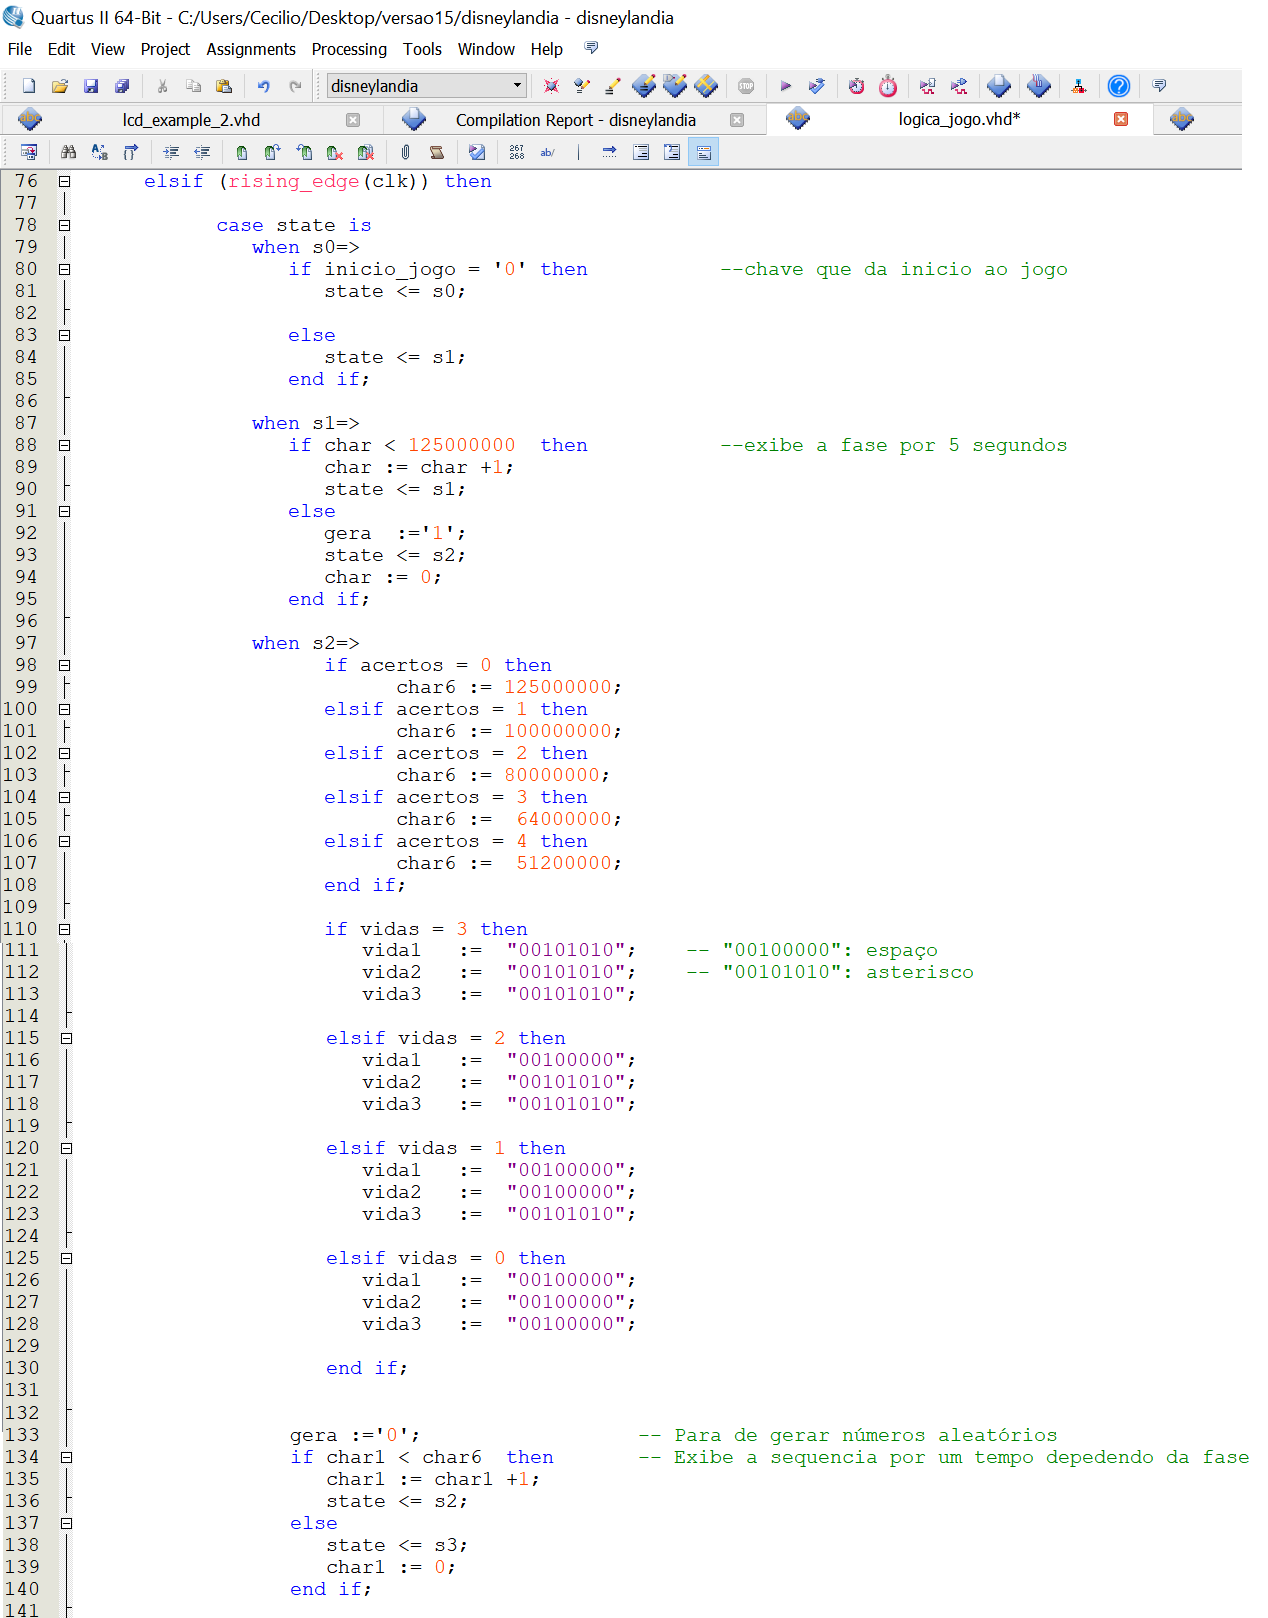
\includegraphics[scale=0.7]{logica_jogo_parte1.png}
                    \caption{Código da Lógica do Jogo - Parte 1}
                    \label{parte1}
                \end{figure}     
                  
                 \begin{figure}[H]
                    \centering
                    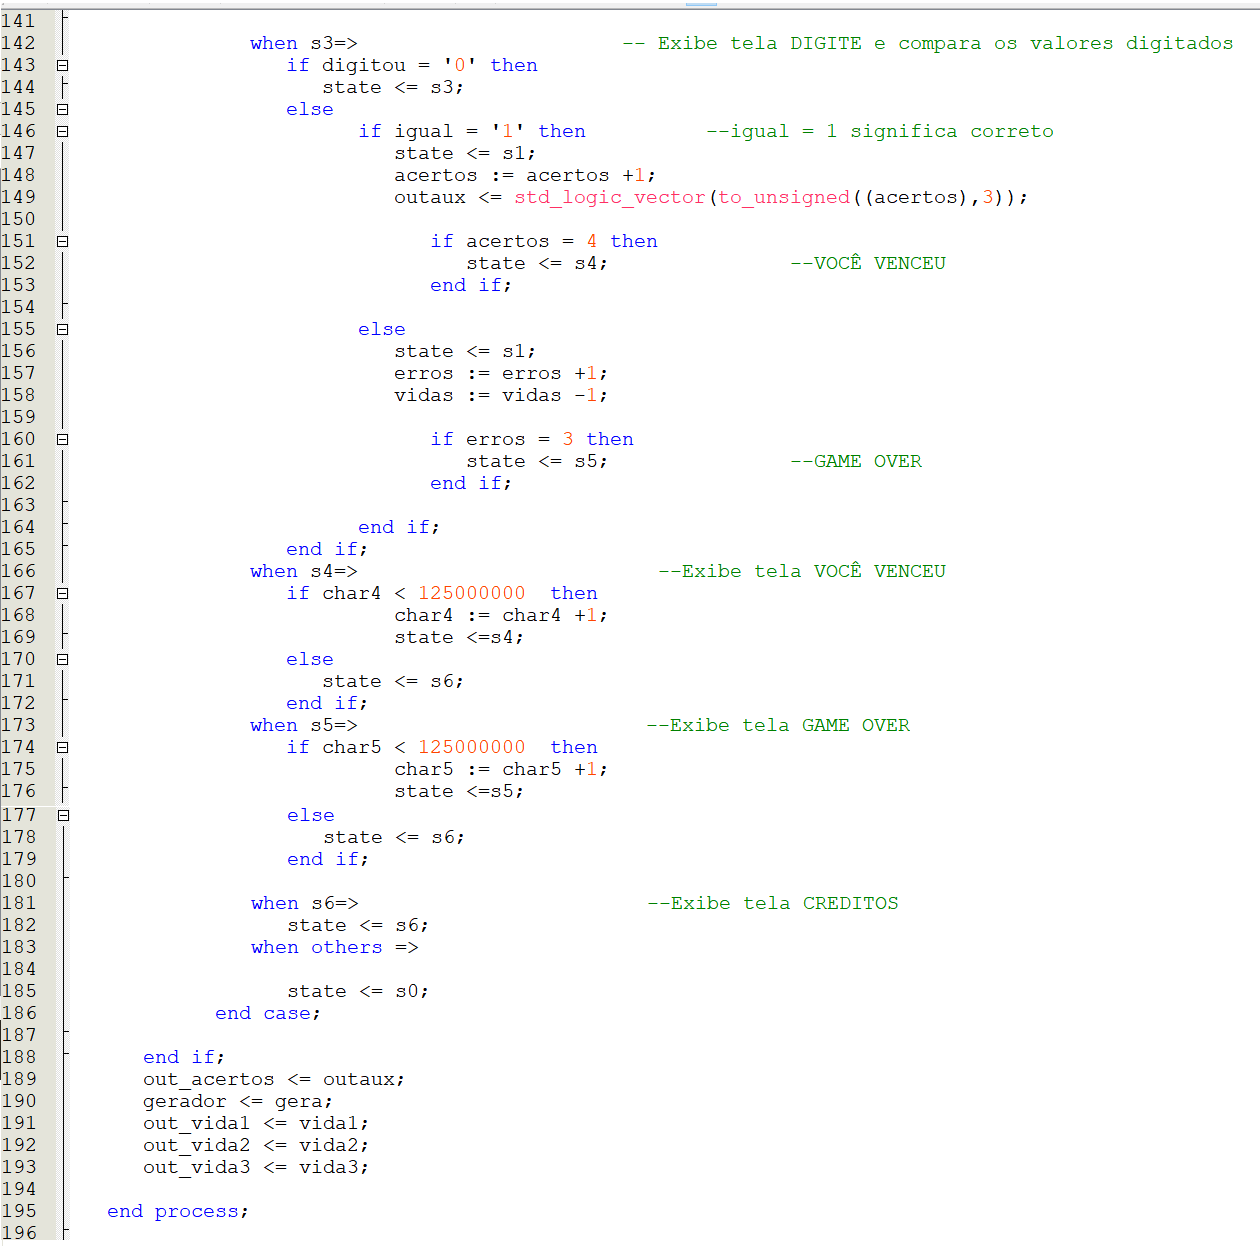
\includegraphics[scale=0.7]{logica_jogo_parte2.png}
                    \caption{Código da Lógica do Jogo - Parte 2}
                    \label{parte2}
                \end{figure}   
                    
                    
               
               
               
                
            \section[Infravermelho]{\hyperlink{toc}{Infravermelho}}
                \tab  O sistema de comunicação entre o controle e a placa segue uma sequência previamente informada através do material de embasamento teórico para esta prática. Primeiramente, é importante lembrar que o sistema de recepção de sinal da placa inverte o sinal lógico emitido pelo controle. Assim, quando o controle envia um sinal de nível lógico alto, a placa interpreta como um sinal de nível lógico baixo, e vice-versa. Este ponto é relevante porque o código implementado no recente projeto interpreta os sinais do controle invertidos. Idealizou-se assim, fundamentada no material teórico fornecido, uma máquina de estados atrelada a um contador. Esta máquina possui dois estados iniciais que verificam se o sinal convertido, após o sensor de infravermelho, atende às especificações. O último estado, por sua vez, realiza contagens sucessivas que indicam quanto tempo o sinal recebido e convertido permanece em nível lógico alto. Assim, quando este sinal passa a ser de nível lógico baixo, comandos condicionais auxiliam no preenchimento de um vetor que será destinado à saída do bloco. Ainda, um comando foi usado para informar ao sistema exterior que uma tecla indesejada do controle foi pressionada. Desta forma, o código de outro bloco pode repudiar quaisquer sinais referentes às demais teclas, assimilando apenas as que vão do algarismo 0 ao 9. \\
                \tab Observa-se na Figura \ref{fig:infra} a implementação do Módulo do Controle Infravermelho.
                \begin{figure}[H]
                    \centering
                    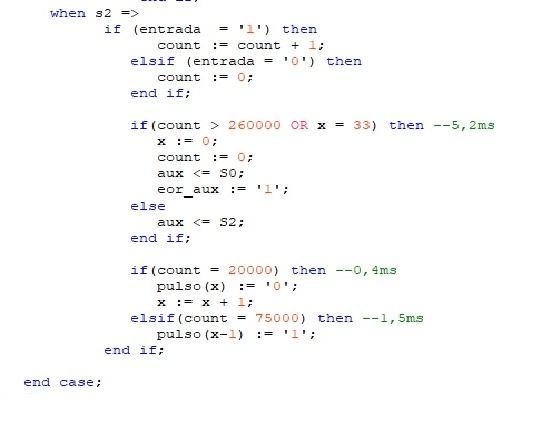
\includegraphics[scale=0.8]{3estado.png}
                    \caption{O terceiro estado (S2) é responsável por registrar os valores no vetor de saída.}
                    \label{fig:infra}
                \end{figure}.\\
                \begin{figure}[H]
                    \centering
                    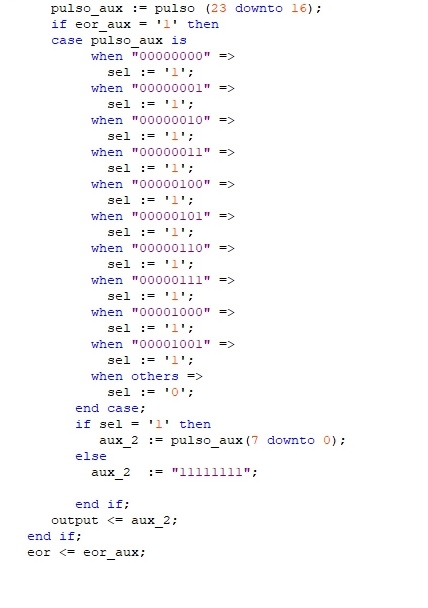
\includegraphics[scale=0.8]{case.png}
                    \caption{Se a tecla pressionada no controle for diferente dos números 0-9, o vetor de saída recebe uma sequência de 1.}
                    \label{figura}
                \end{figure} \\
                \tab Ainda, vale observar os sinais enviados pelo controle remoto para o sensor da placa. O sinal começa com um pulso de 9 ms (4,6 ms é o suficiente) e é seguido por um espaço de 4,5 ms (4,2 ms é o suficiente). Em seguida, uma sequência de pulsos e espaços, com intervalos de tempo entre 0,4 ms e 1,5 ms, fornece as informações necessárias para preencher o vetor de saída. Lembrando que os valores recebidos pela placa já estão invertidos. Assim, a análise feita acima deve levar em conta que o sensor inverterá os sinais em questão.\\
                \begin{figure}[H]
                    \centering
                    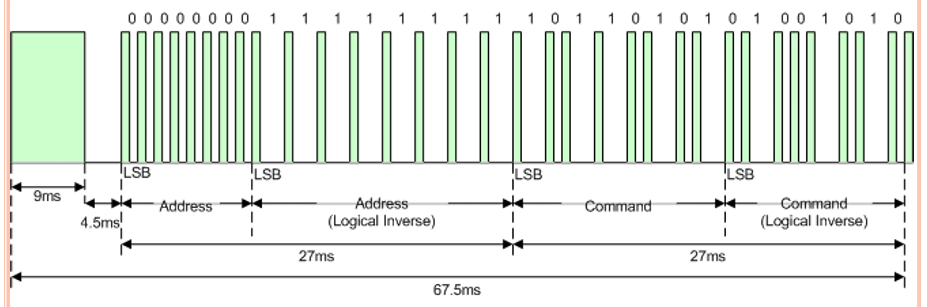
\includegraphics[scale=0.6]{grafico.png}
                    \caption{O gráfico temporal mostra os sinais enviados pelo controle remoto.}
                    \label{figura}
                \end{figure}
            \section[Random]{\hyperlink{toc}{Random}}
                \tab O módulo \textbf{Random} pussui duas funções principais. A primeira consiste em gerar o número aleatório que será exibido para o jogador e a segunda consiste em receber o número digitado pelo jogador e compara-lo com o número gerado e determinar se a sequência foi digitada corretamente.
                
                \subsection{Gerador de Números Aleatórios}
                    \tab Aqui encontramos um dilema, computação convencional não gera números aleatórios, pois é baseada em princípios fisícos clássicos e na fisíca classica não existem processos intrinsecamente aleatórios, sendo a aparente aleatoriedade gerada pela ignorância acerca do sistema. Sendo assim baseamos a geração de números aleatorios no clock da máquina, pois sendo este muito rápido e com uma seleção por comando manual em um momento selecionado inconcientemenete pelo jogador o processo se torna satisfatóriamente aleatótio . Ainda com isso precisamos de 8 numéros aleatórios então damos um tratamento ao número obtido no processo descrito anteriormente por uma gama de equações, estas sim selecionadas aleatóriamente, para que se obtenha valores distintos pseudo aleatórios .
                    
                    \tab O código referente a essa lógica pode ser visto na Figura \ref{random_aleatorio}.
                    
                        \begin{figure}[H]
                         \centering                    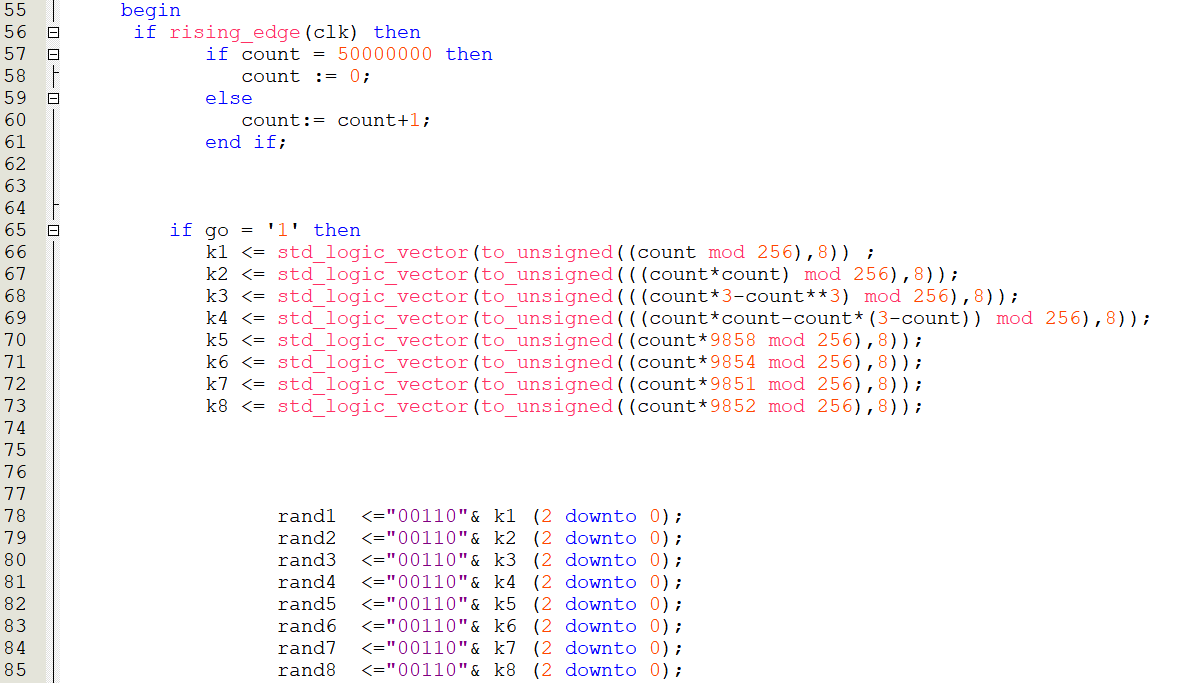
\includegraphics[scale=0.6]{random_aleatorio.png}
                         \caption{Código da parte de geração de sequências aleatórias do módulo \textbf{Random}}
                         \label{random_comparador}
                        \end{figure} \\
                        
                
                \subsection{Comparador}
                    \tab Nessa parte do código, inicialmente, atribui-se cada valor digitado pelo jogador às 8 variáveis distintas, em seguida usa-se oito variáveis para acender os LED indicadores e, por último, compara-se os quatro últimos bits da sequência gerada com a sequência digitada. \\
                    \tab O código referente a essa lógica pode ser visto na Figura \ref{random_comparador}.\\
                    
                    \begin{figure}[H]
                     \centering                    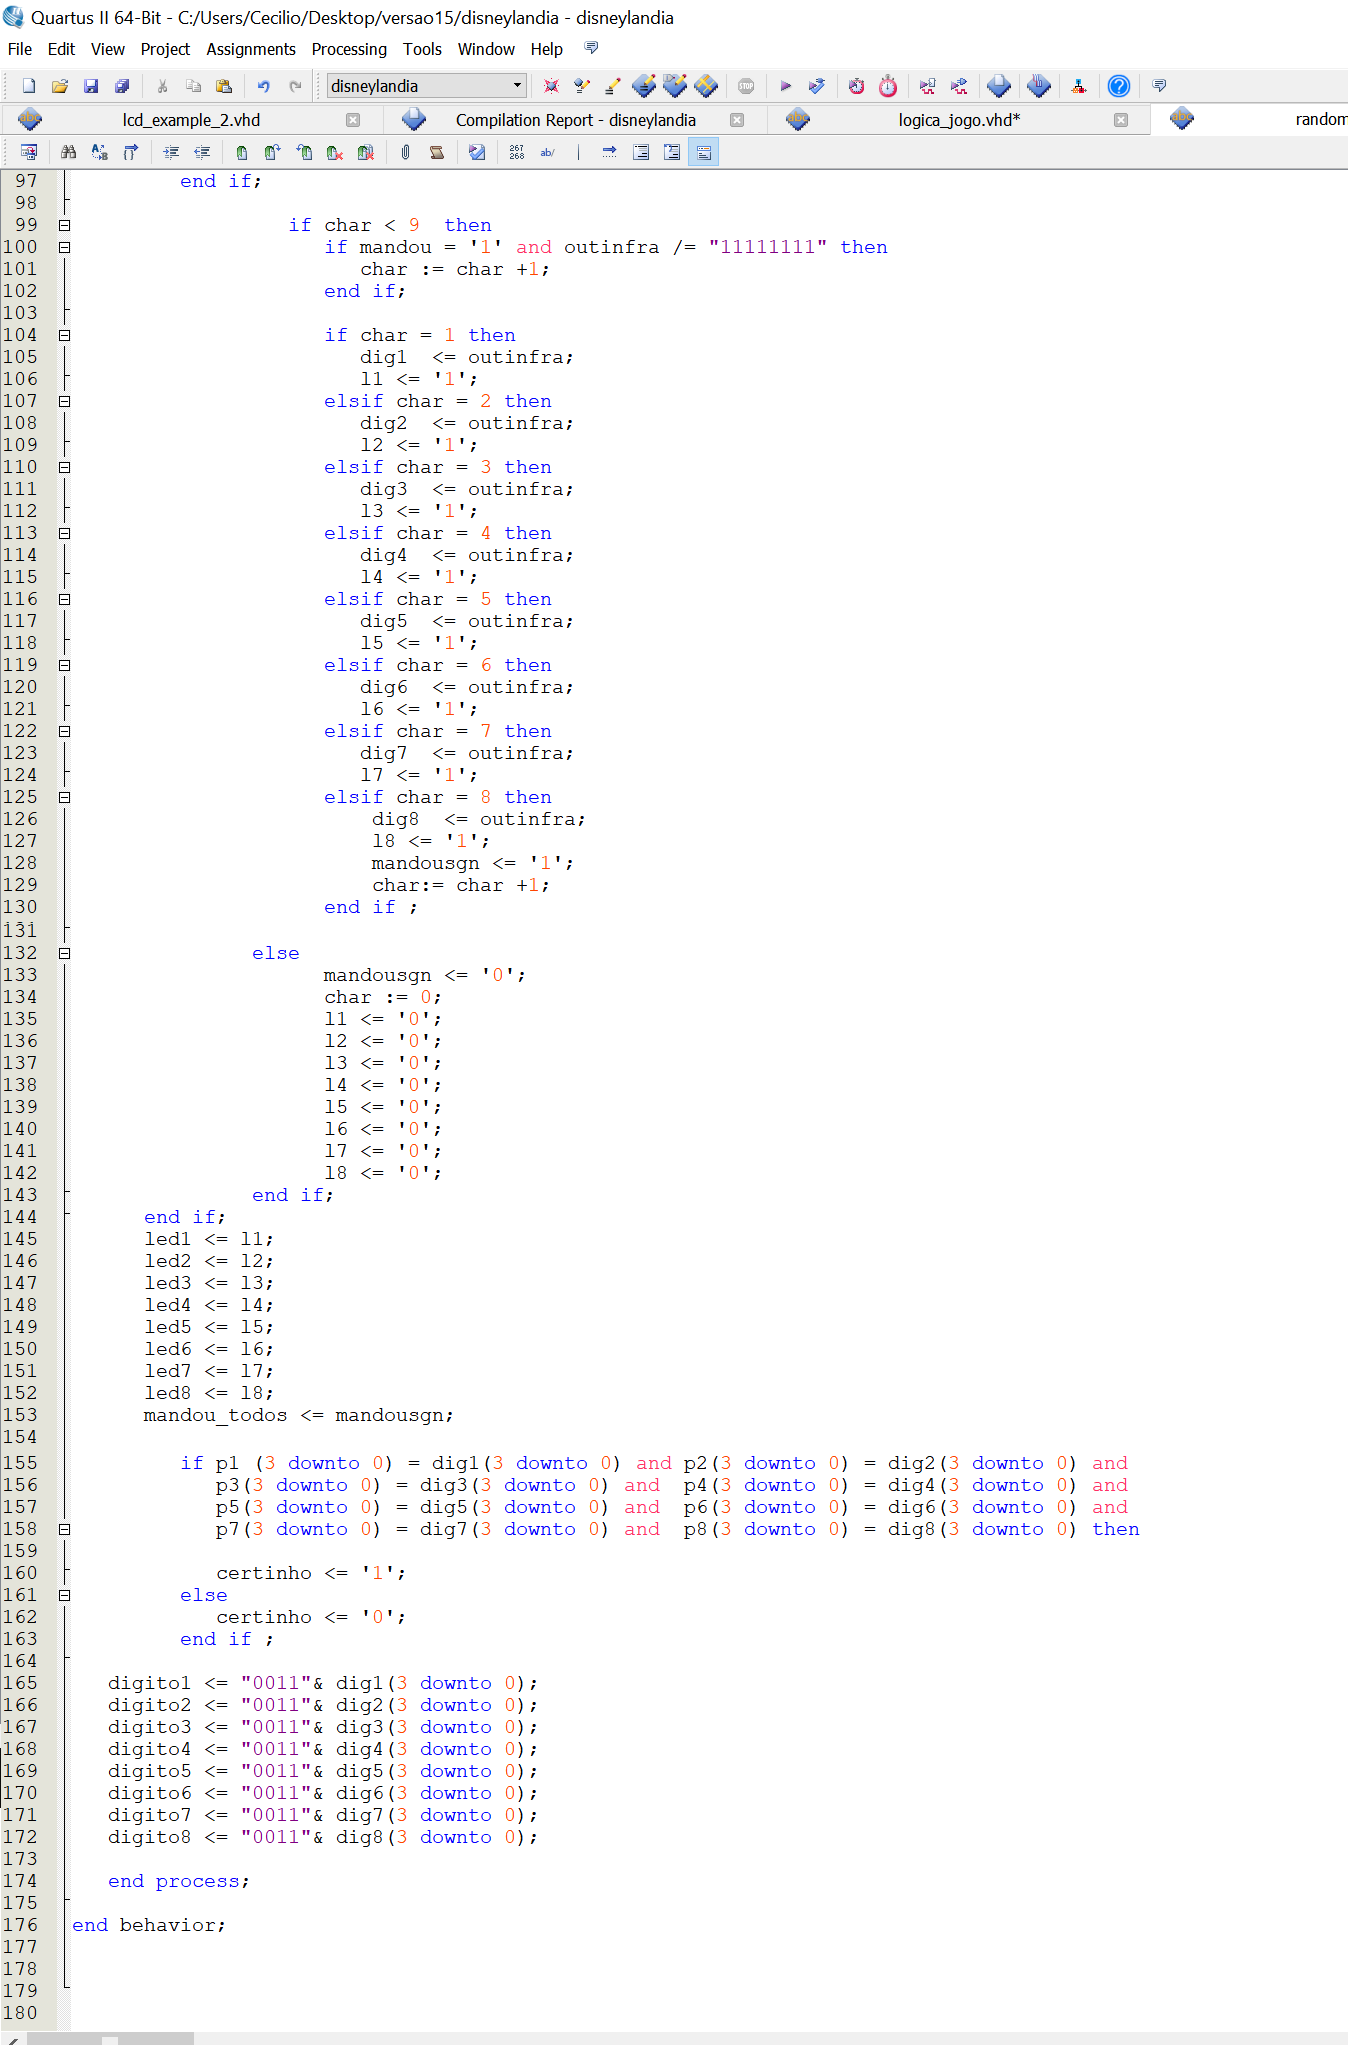
\includegraphics[scale=0.6]{random_comparador.png}
                     \caption{Código da parte de comparação do módulo \textbf{Random}}
                     \label{random_comparador}
                    \end{figure} \\
                
                
         \chapter[Manual de Operação]{\hyperlink{toc}{Manual de Operação}}
                \tab Esta seção é dedicada a esclarecer o funcionamento e organização da placa da \textit{Altera DE2-115}, bem como explicitar quais chaves, displays, LEDs e botões foram utilizados na implementação do jogo de repetição. \\
                \tab Observa-se um esquemático da placa na Figura \ref{manual}. Em que:
              
                \begin{itemize}
                    \item SW[7] corresponde a chave que dá início ao jogo. 
                    \item Exibe-se as mensagens do jogo no LCD.
                    \item O receptor recebe os sinais do controle remoto.
                    \item LEDR[0] a LEDR[7] indicam que o jogador digitou um número.
                \end{itemize} \\
                
                \begin{figure}[H]
                    \centering                    
                    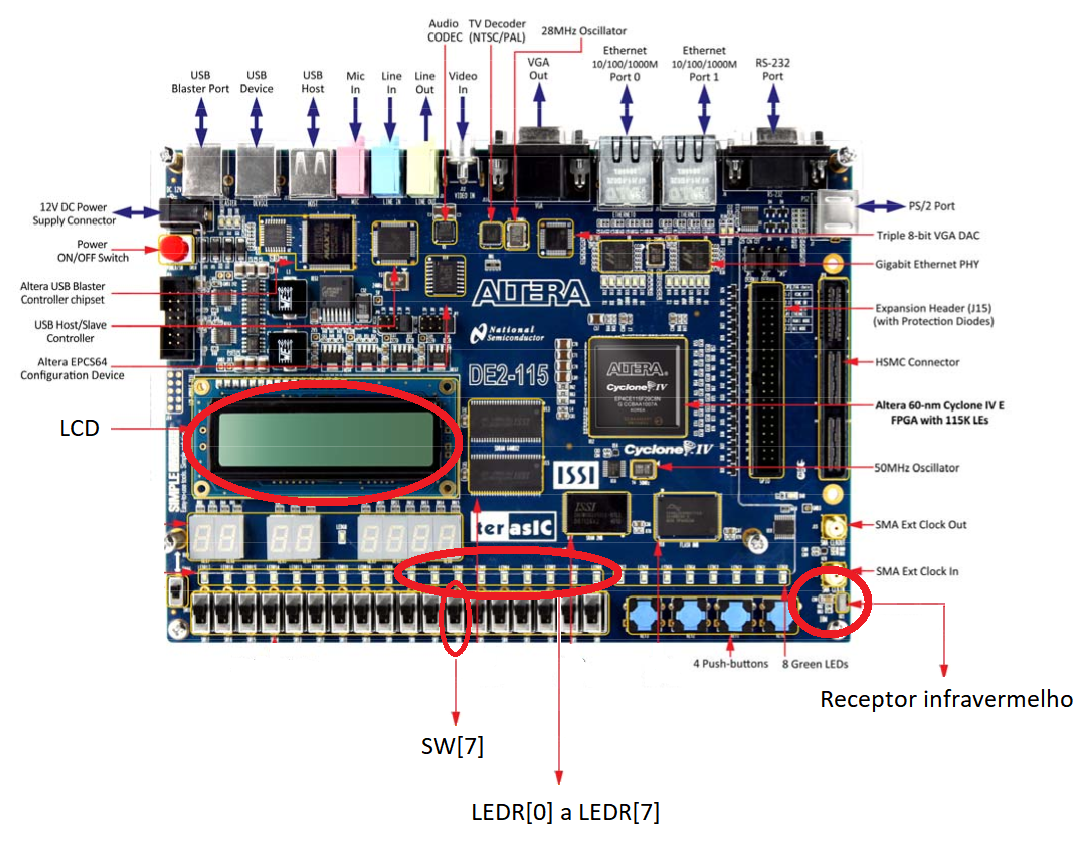
\includegraphics[width=\columnwidth]{manual.png}
                    \caption{Manual de Operação}
                    \label{manual}
                \end{figure} \\
                
         
         \chapter[Resultados]{\hyperlink{toc}{Resultados}}
            
            \tab Observa-se a seguir imagens de simulações, usando a ferramenta \textit{University Program VWF}, da lógica do jogo e fotos da placa operando nos diferentes estados da Maquina de Estados que guiam a lógica do jogo. \\
            \tab Nas Figuras \ref{acertou} e \ref{errou}, observam-se simulações de jogos em que o jogador acertou todas as sequências e que o jogador errou todas as sequência, respectivamente. \\
            
                \begin{figure}[H]
                    \centering
                    \hspace*{-1.5cm} 
                    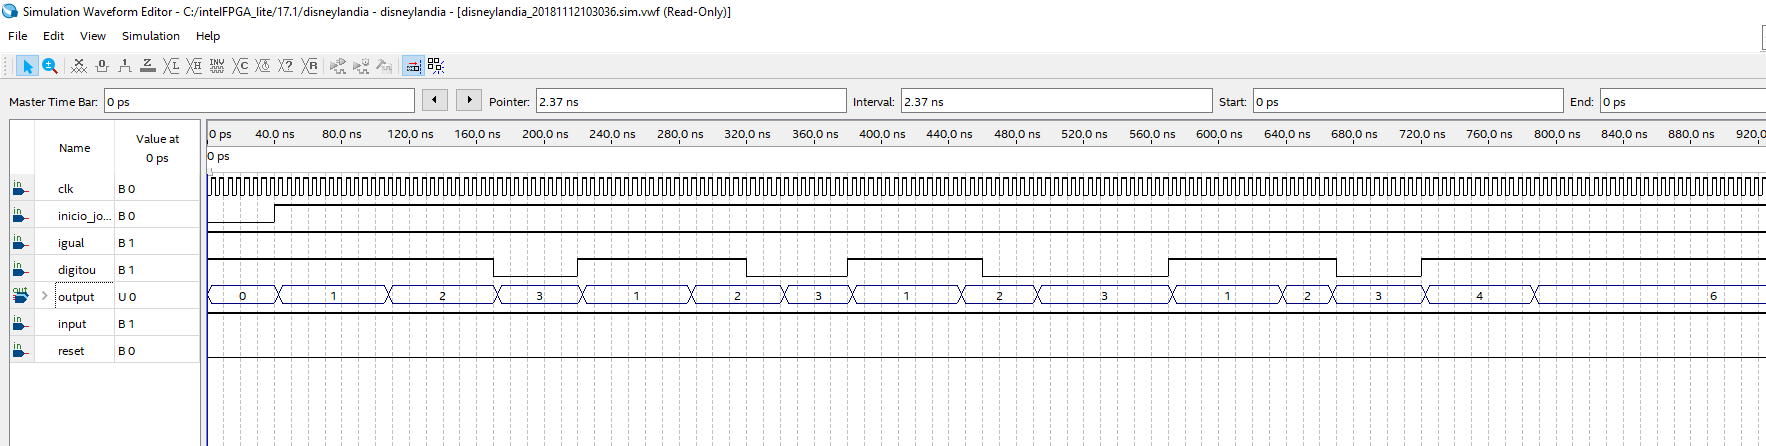
\includegraphics[scale=0.41]{logica_jogo_acertou_zoom.png}
                    \caption{Simulação de jogo em que o jogador acertou todas as sequências}
                    \label{acertou}
                \end{figure} \\
                
                \begin{figure}[H]
                    \centering
                    \hspace*{-1.5cm} 
                    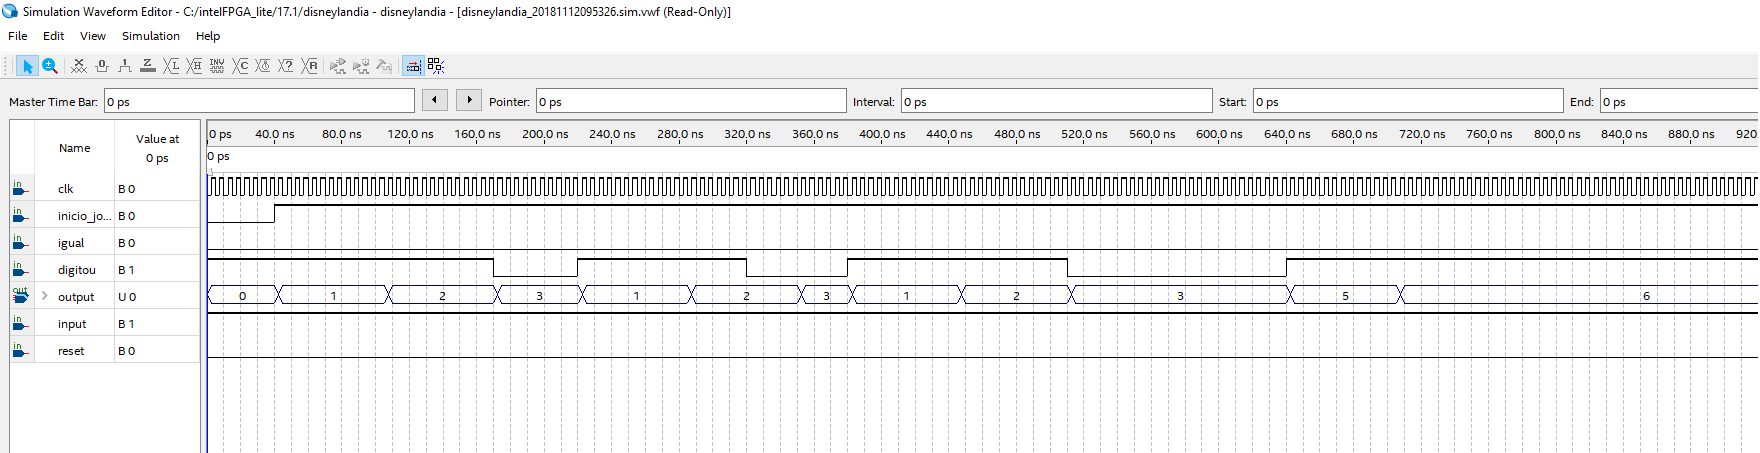
\includegraphics[scale=0.41]{logica_jogo_errou_zoom.png}
                    \caption{Simulação de jogo em que o jogador errou todas as sequências}
                    \label{errou}
                \end{figure}
                
           \tab Nota-se que, na Figura \ref{acertou}, após quatro acertos, a saída corresponde ao estado "VOCÊ VENCEU" \ e, em seguida segue para os créditos. Analogamente, na Figura \ref{errou}, após três erros, a saída corresponde ao estado "GAME OVER"\ e em seguida segue para os créditos. \\
           \tab Nas Figuras \ref{bem vindo}, \ref{fase}, \ref{sequencia}, \ref{digite}, \ref{voce venceu} e \ref{game over} observa-se a placa nos diferentes estados de operação.
           
           
                
            
            
                \begin{figure}[H]
                    \centering
                    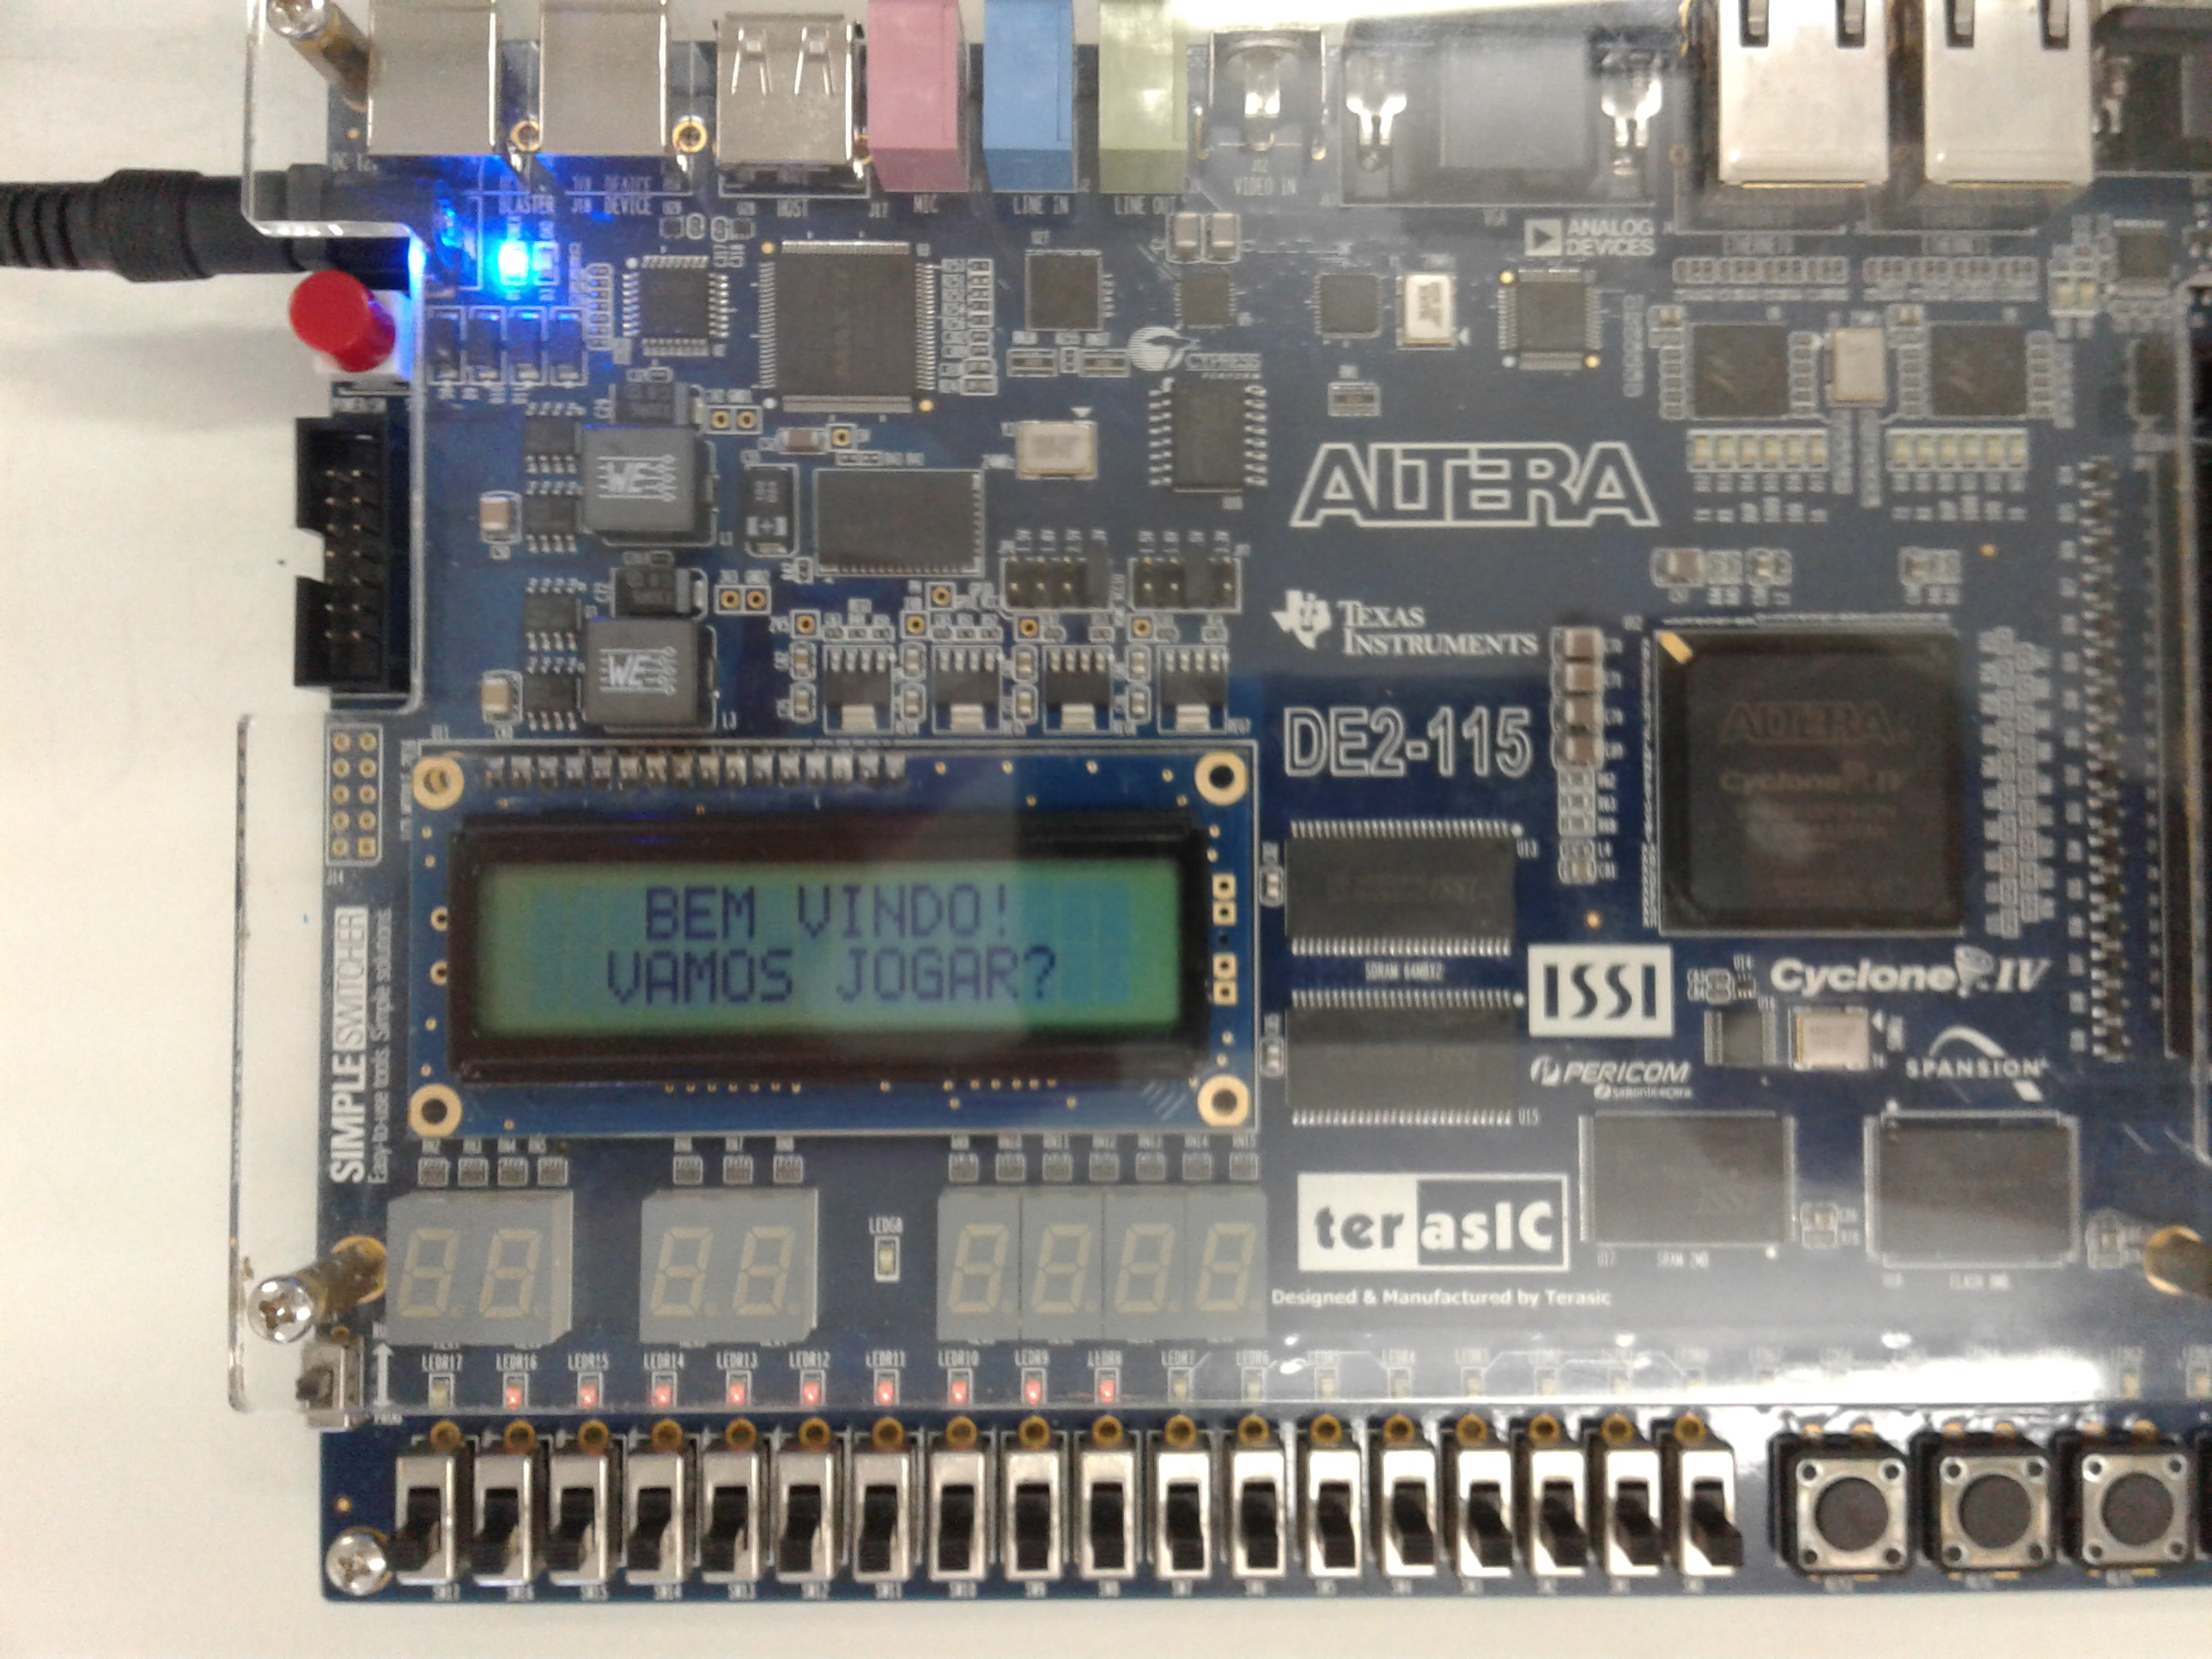
\includegraphics[scale=0.14]{foto_placa_bemvindo.jpg}
                    \caption{Foto da placa operando no estado $S_0$}
                    \label{bem vindo}
                \end{figure}
                
                \begin{figure}[H]
                    \centering
                    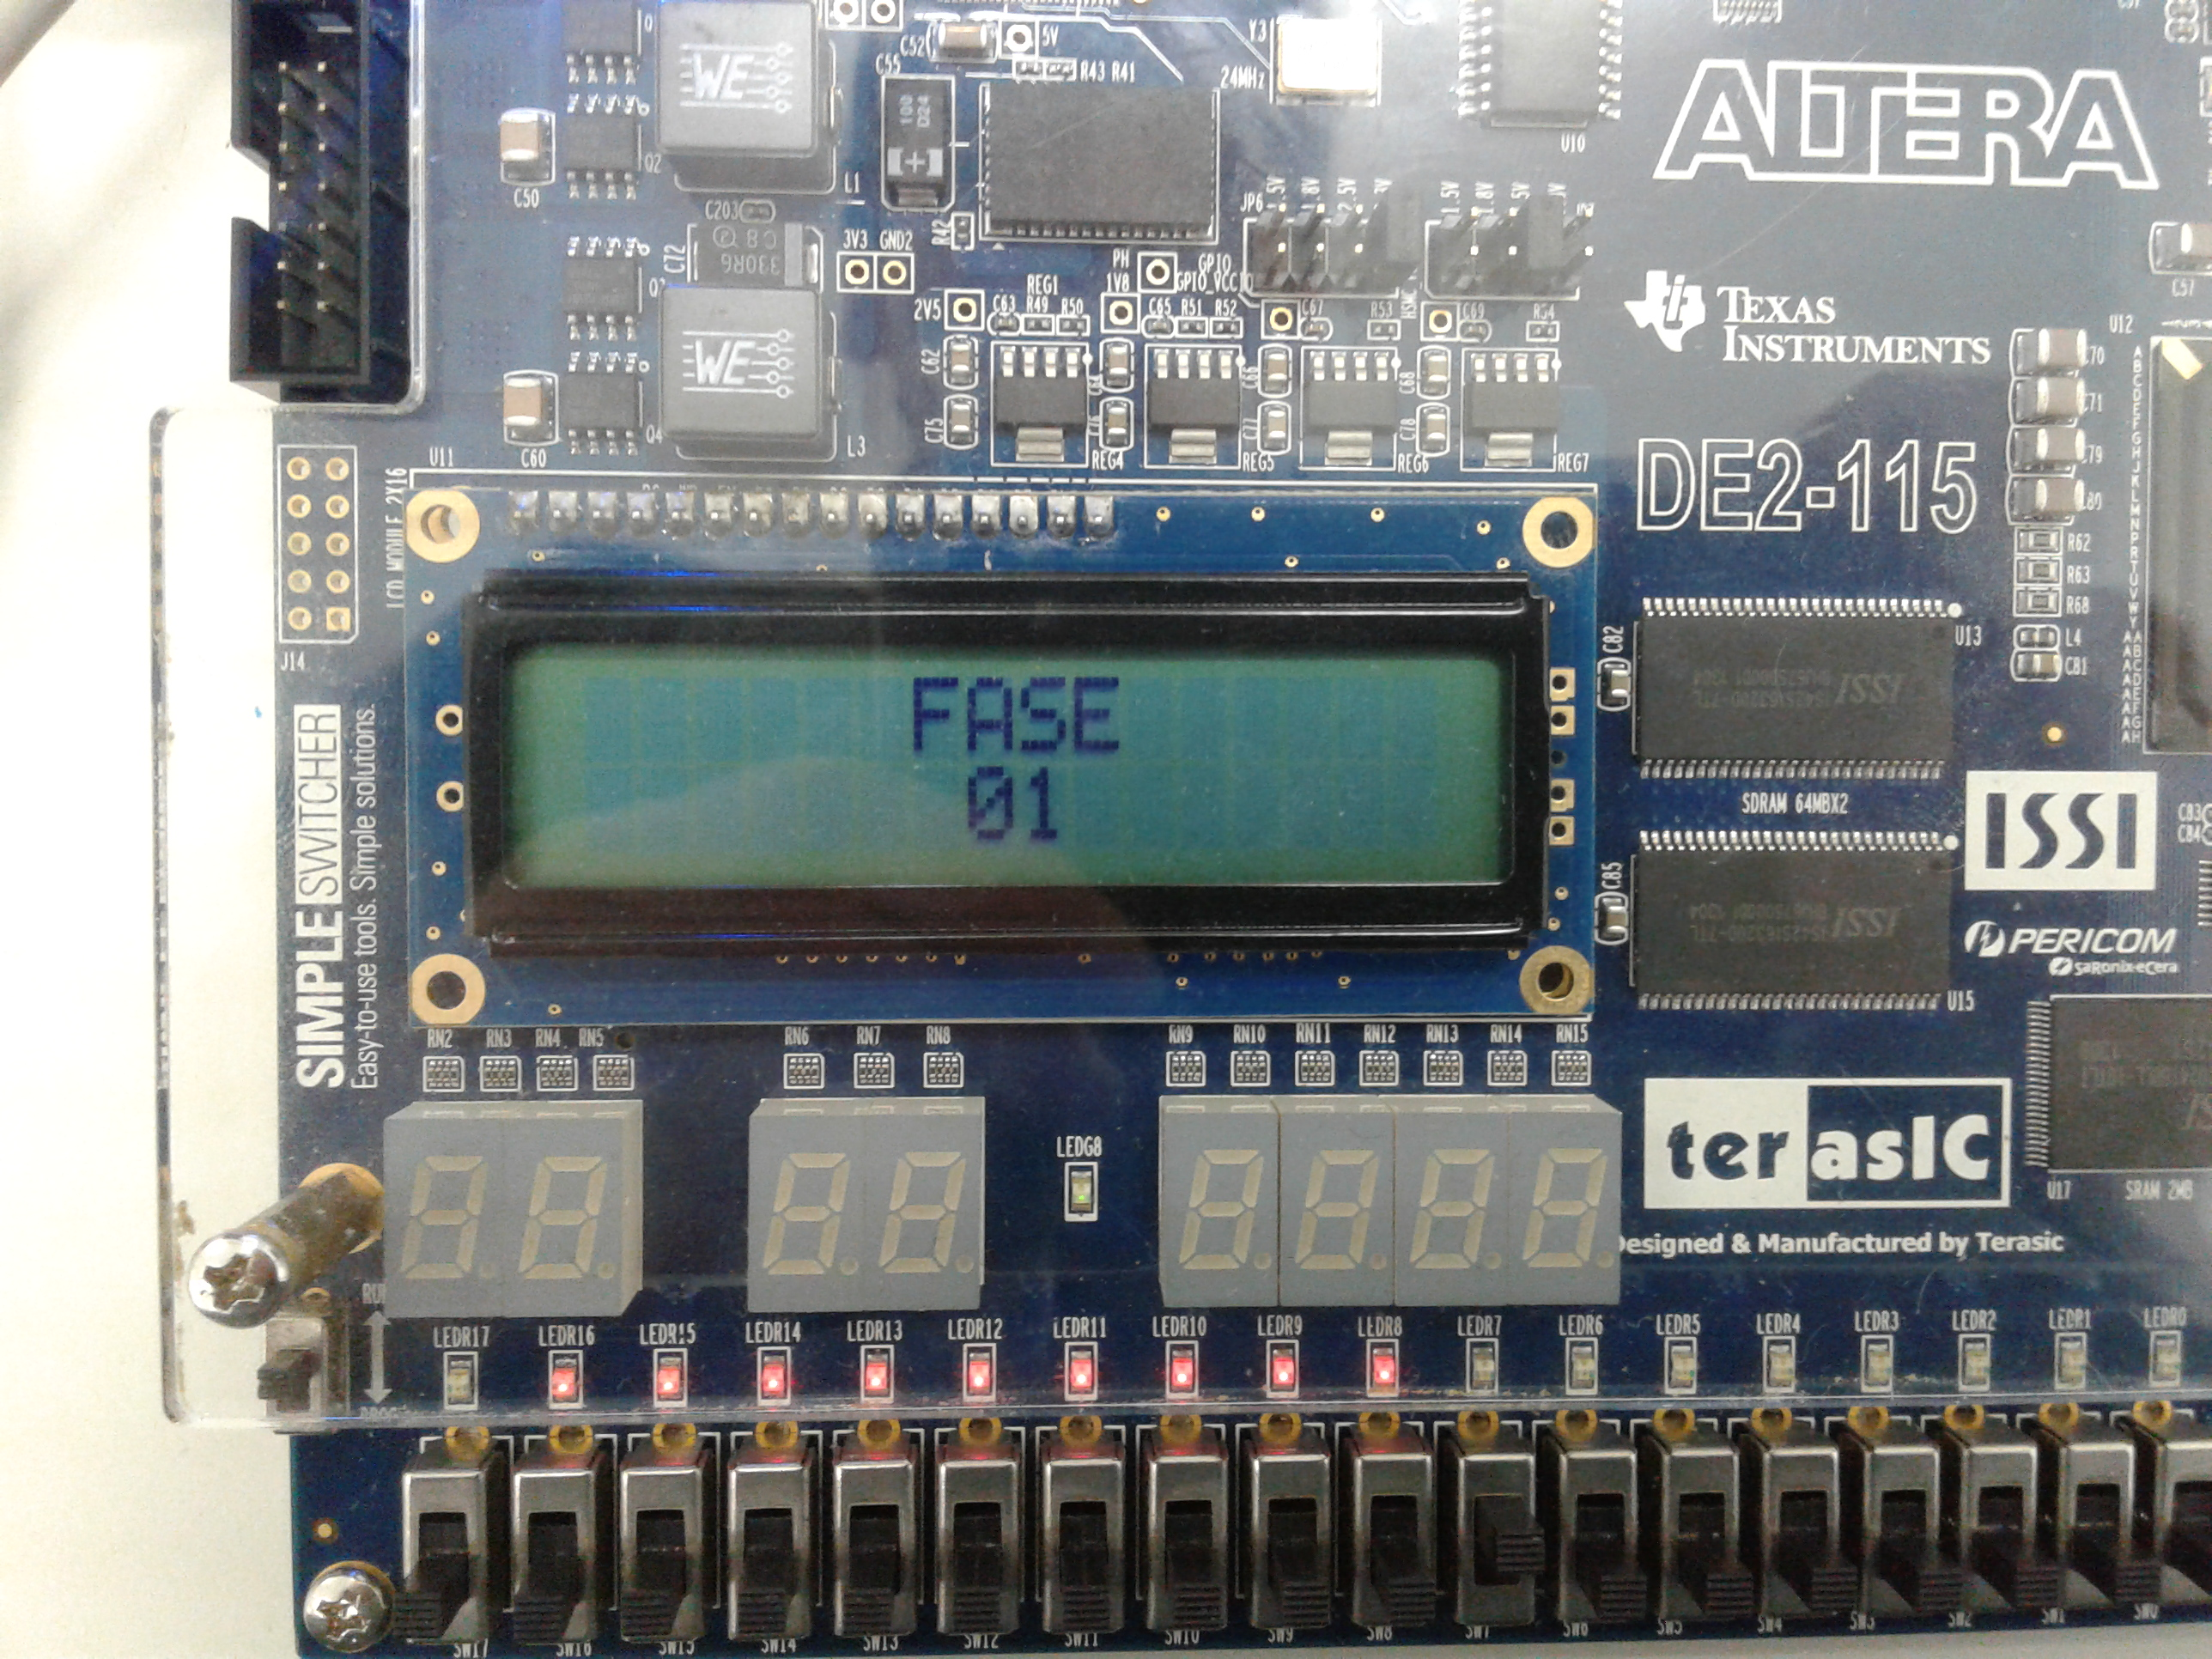
\includegraphics[scale=0.14]{foto_placa_fase.jpg}
                    \caption{Foto da placa operando no estado $S_1$}
                    \label{fase}
                \end{figure}
                
               \begin{figure}[H]
                    \centering
                    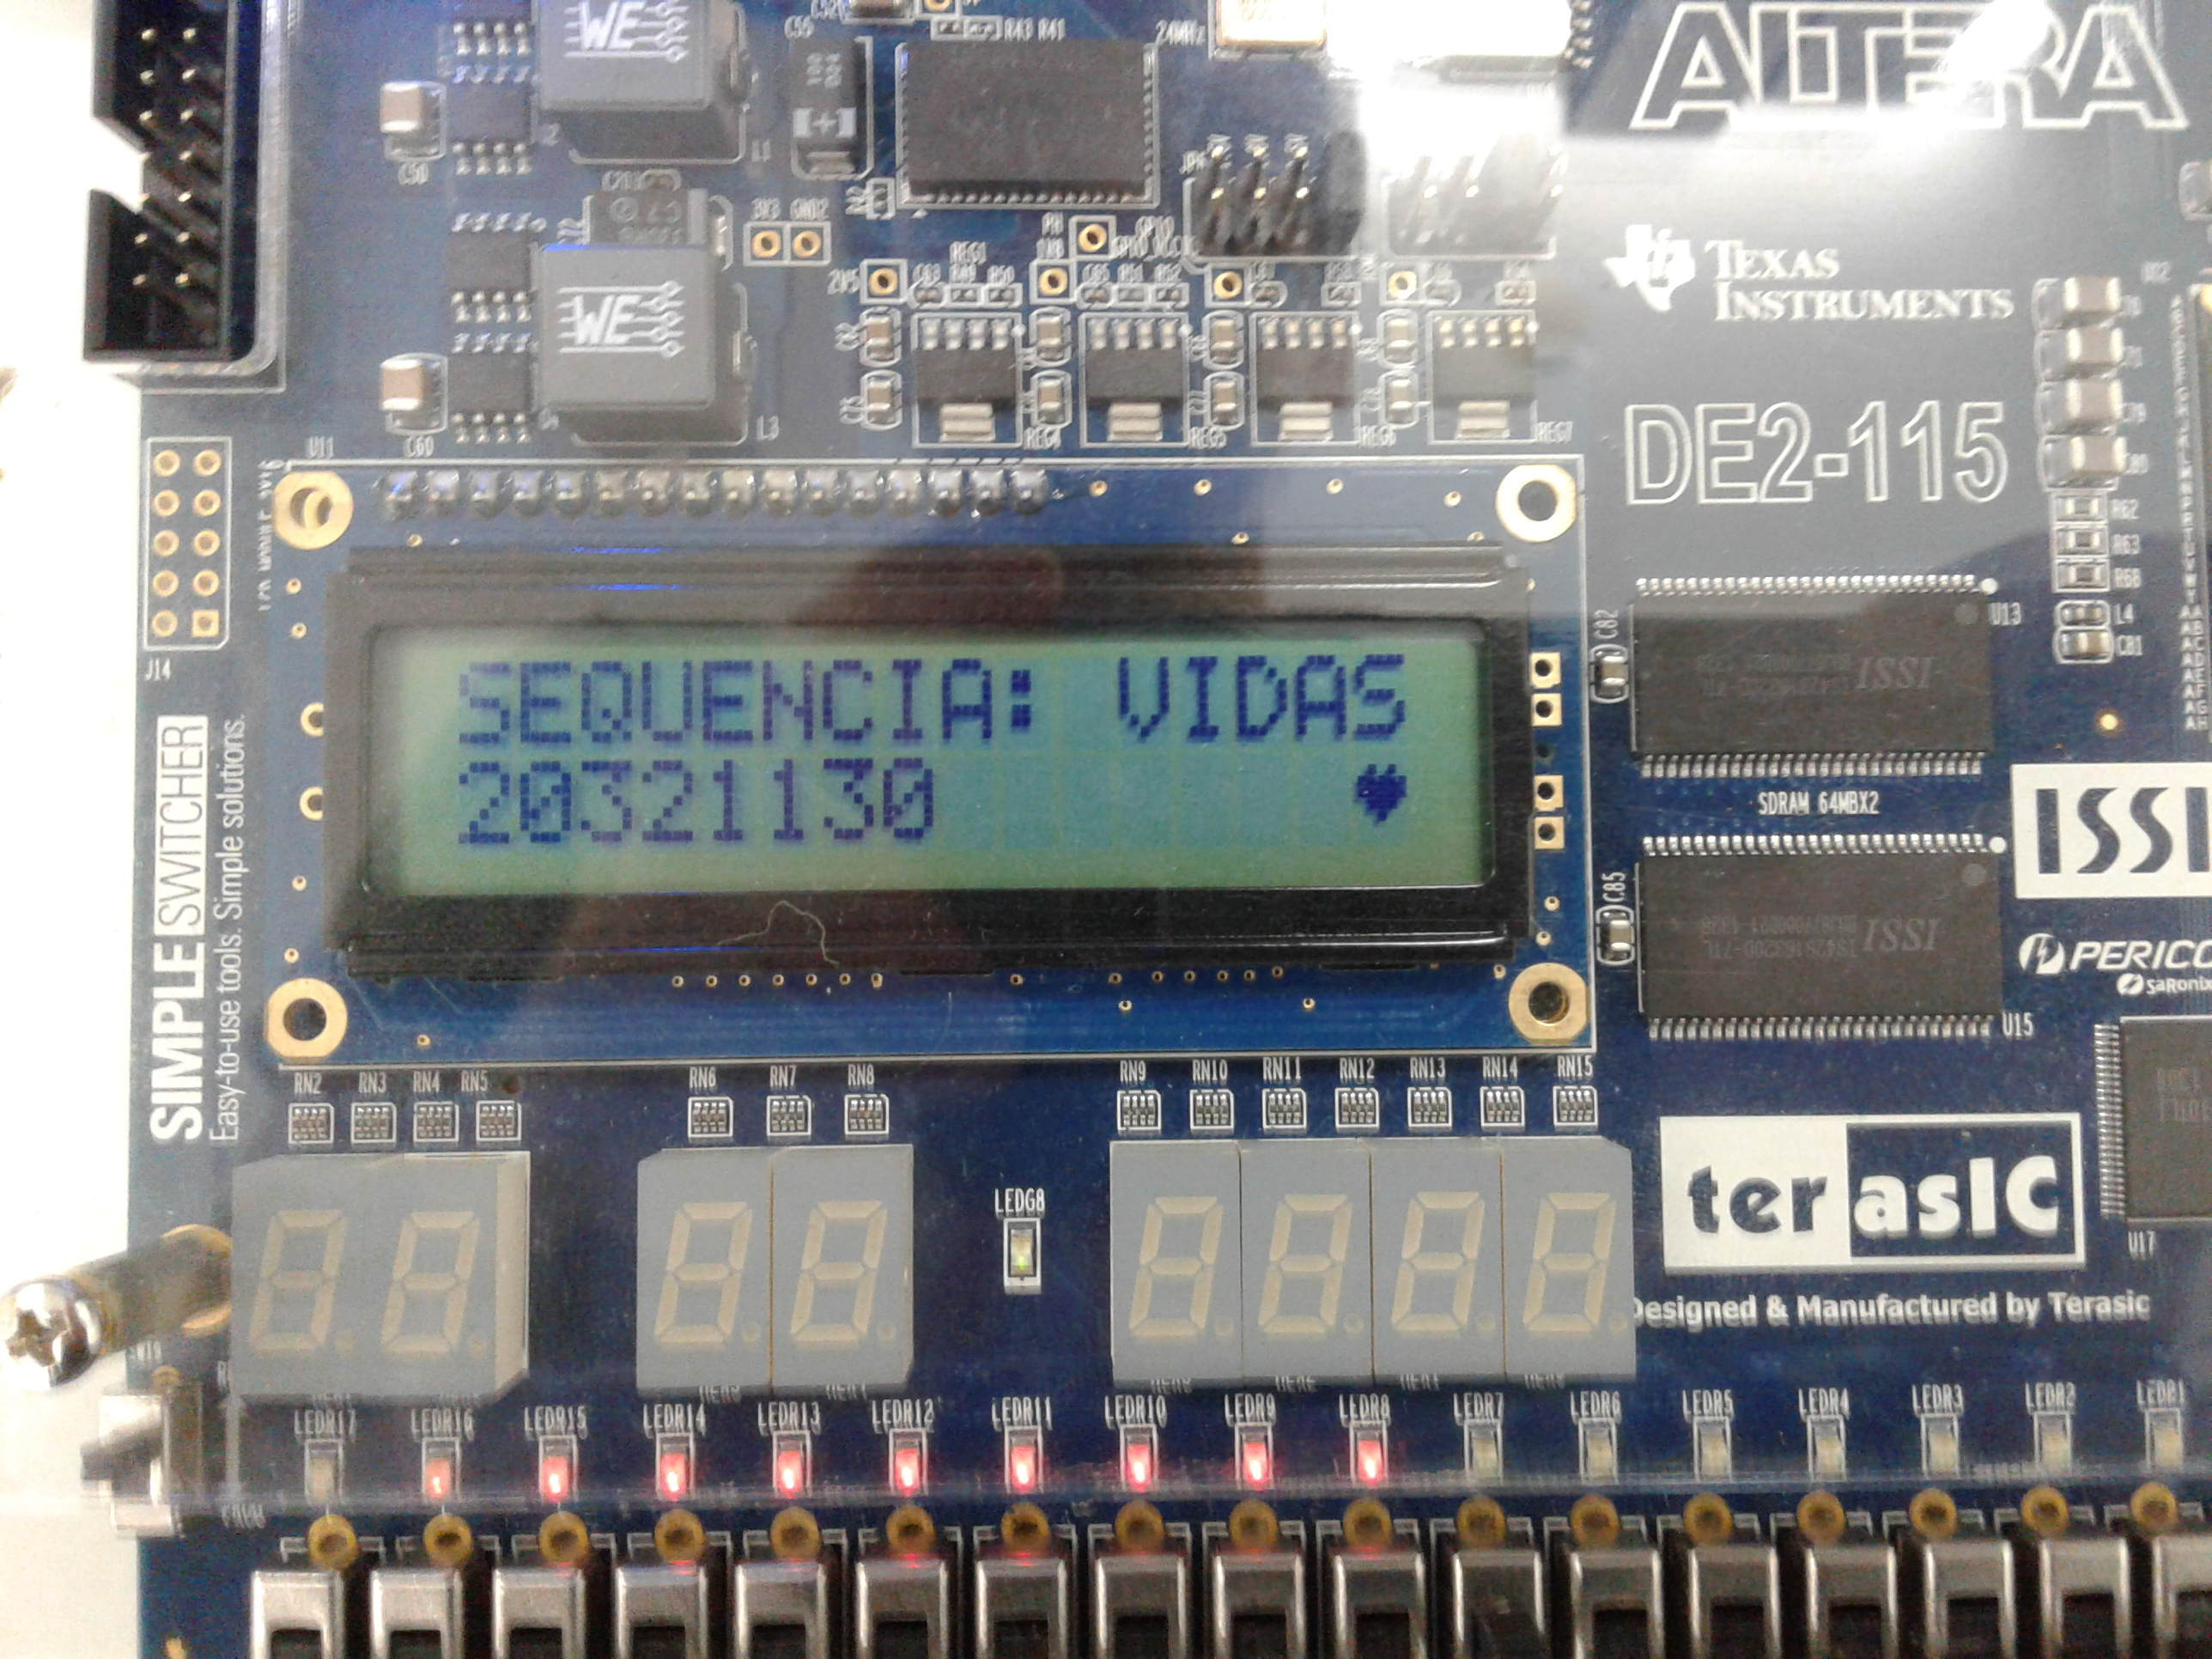
\includegraphics[scale=0.14]{foto_placa_sequencia.jpg}
                    \caption{Foto da placa operando no estado $S_2$}
                    \label{sequencia}
                \end{figure}
                
                 \begin{figure}[H]
                    \centering
                    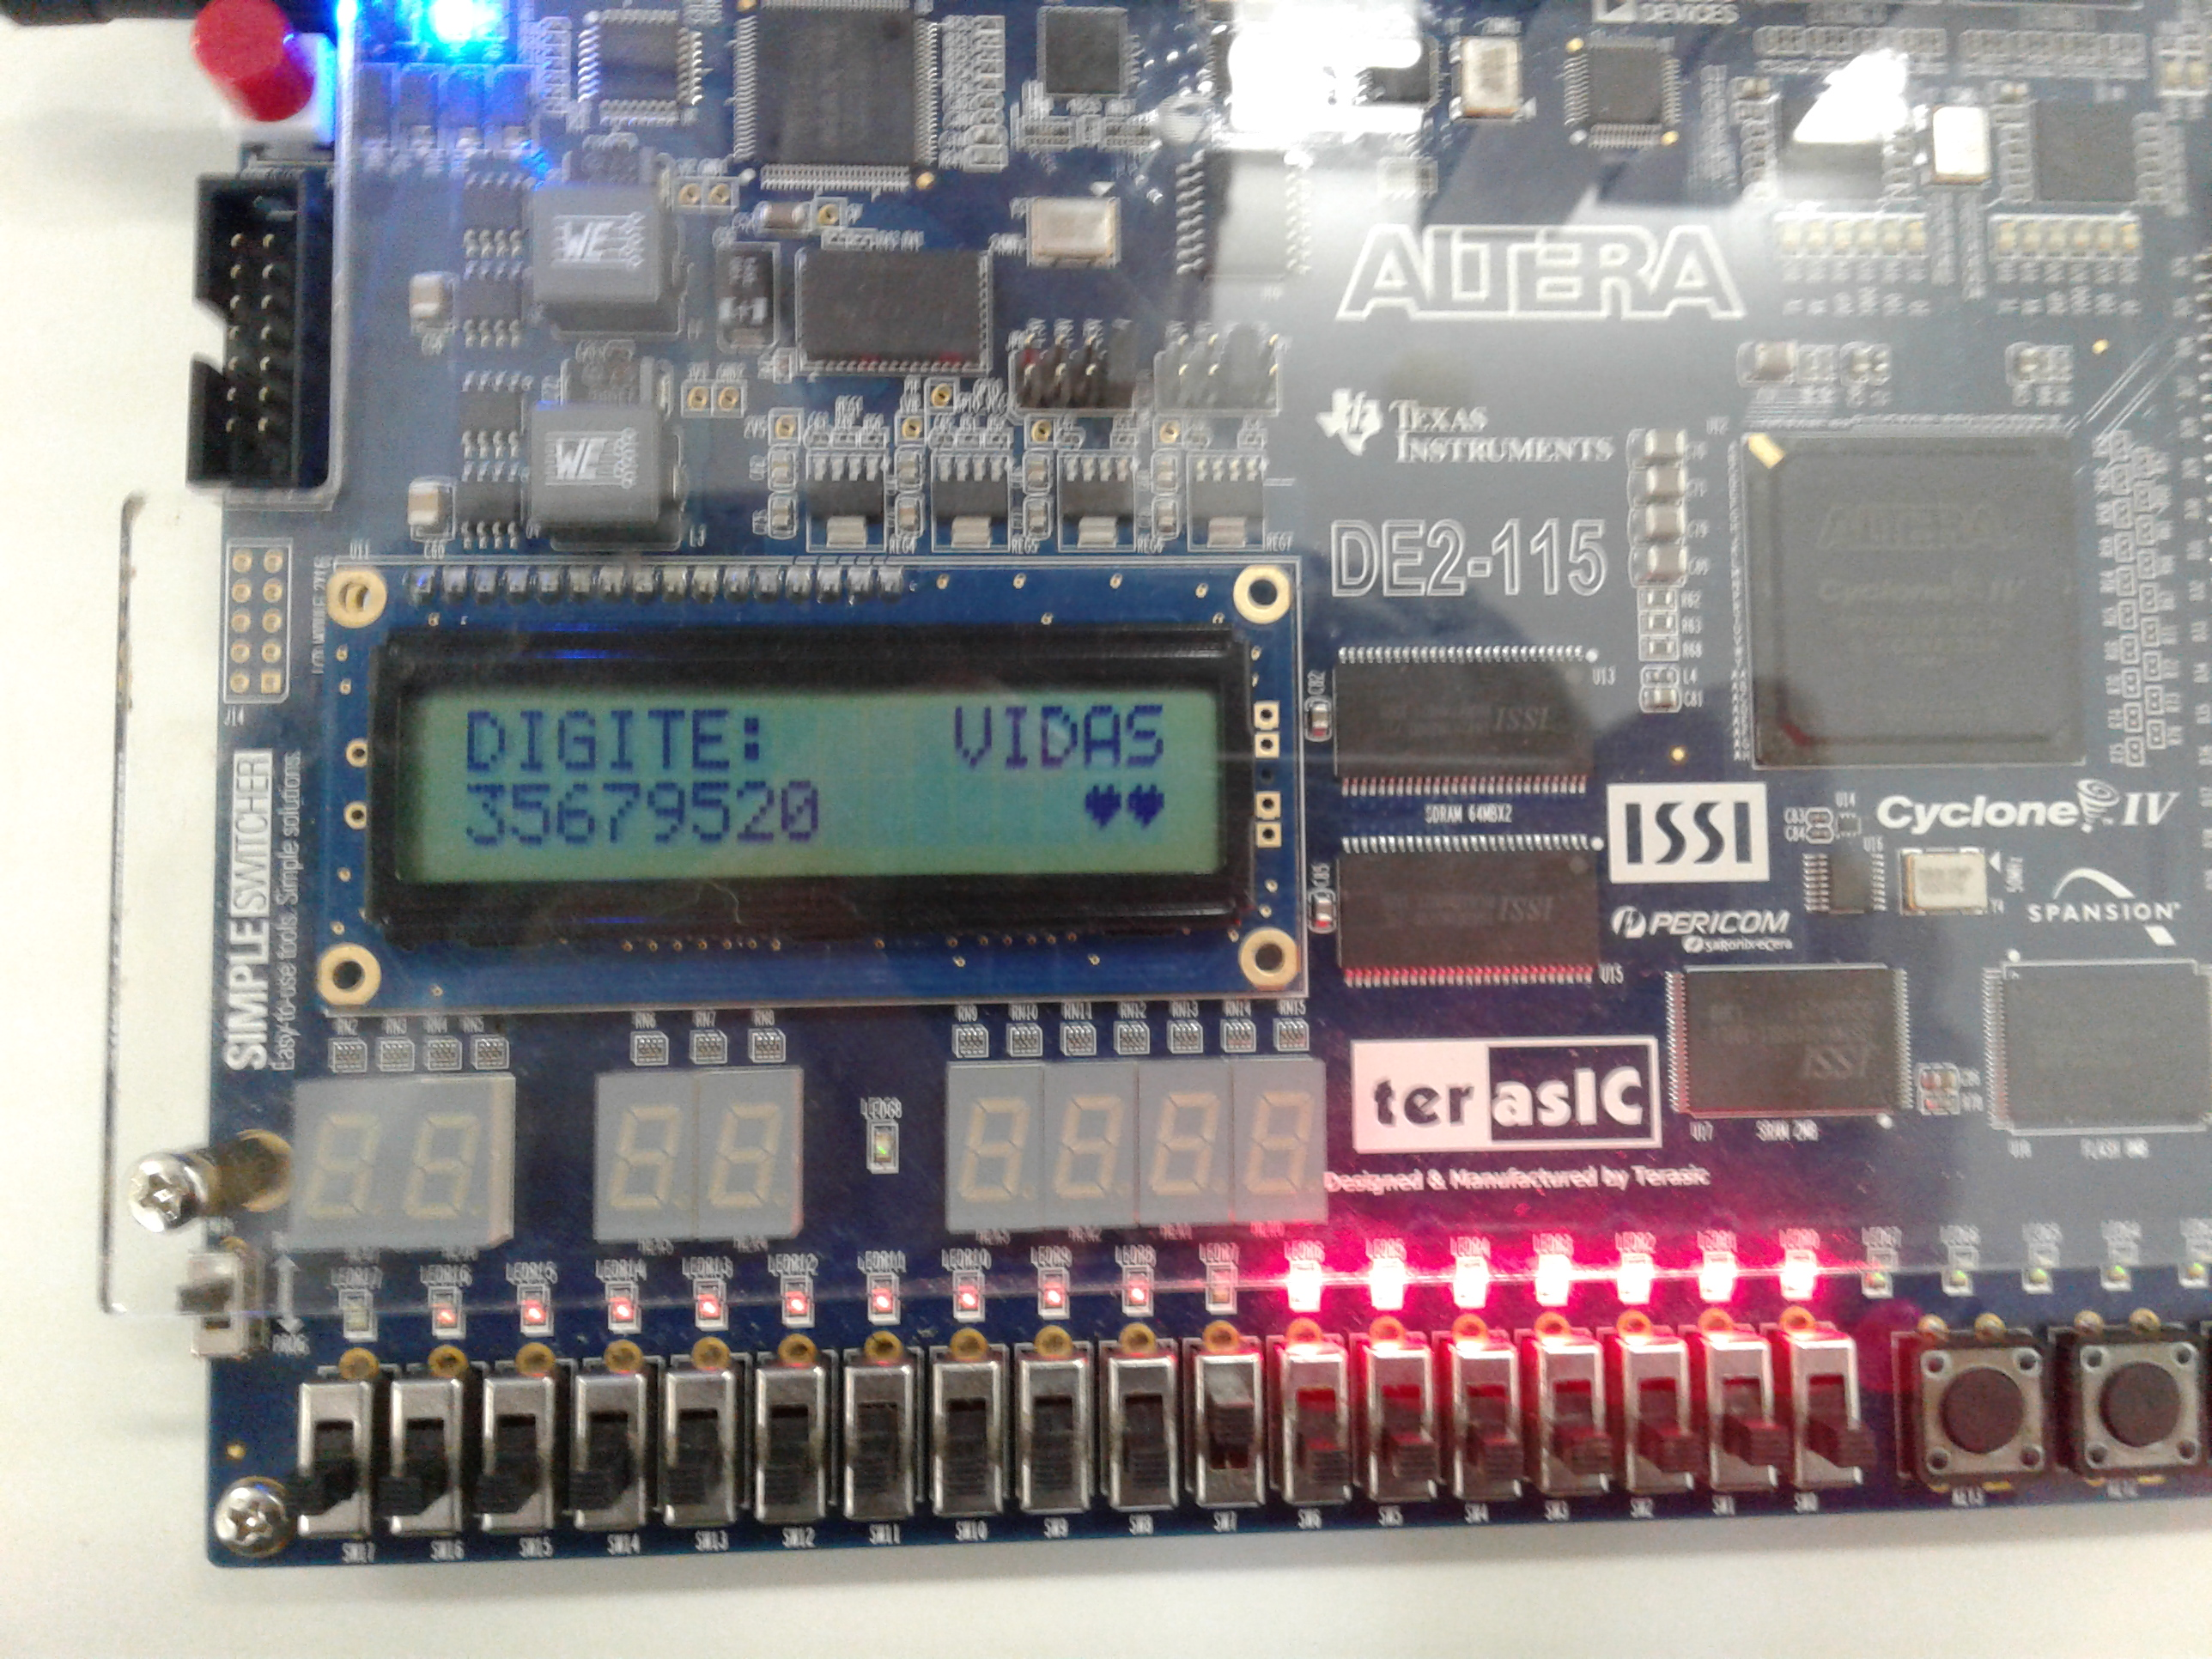
\includegraphics[scale=0.14]{foto_placa_digite.jpg}
                    \caption{Foto da placa operando no estado $S_3$}
                    \label{digite}
                \end{figure}
                
                 \begin{figure}[H]
                    \centering
                    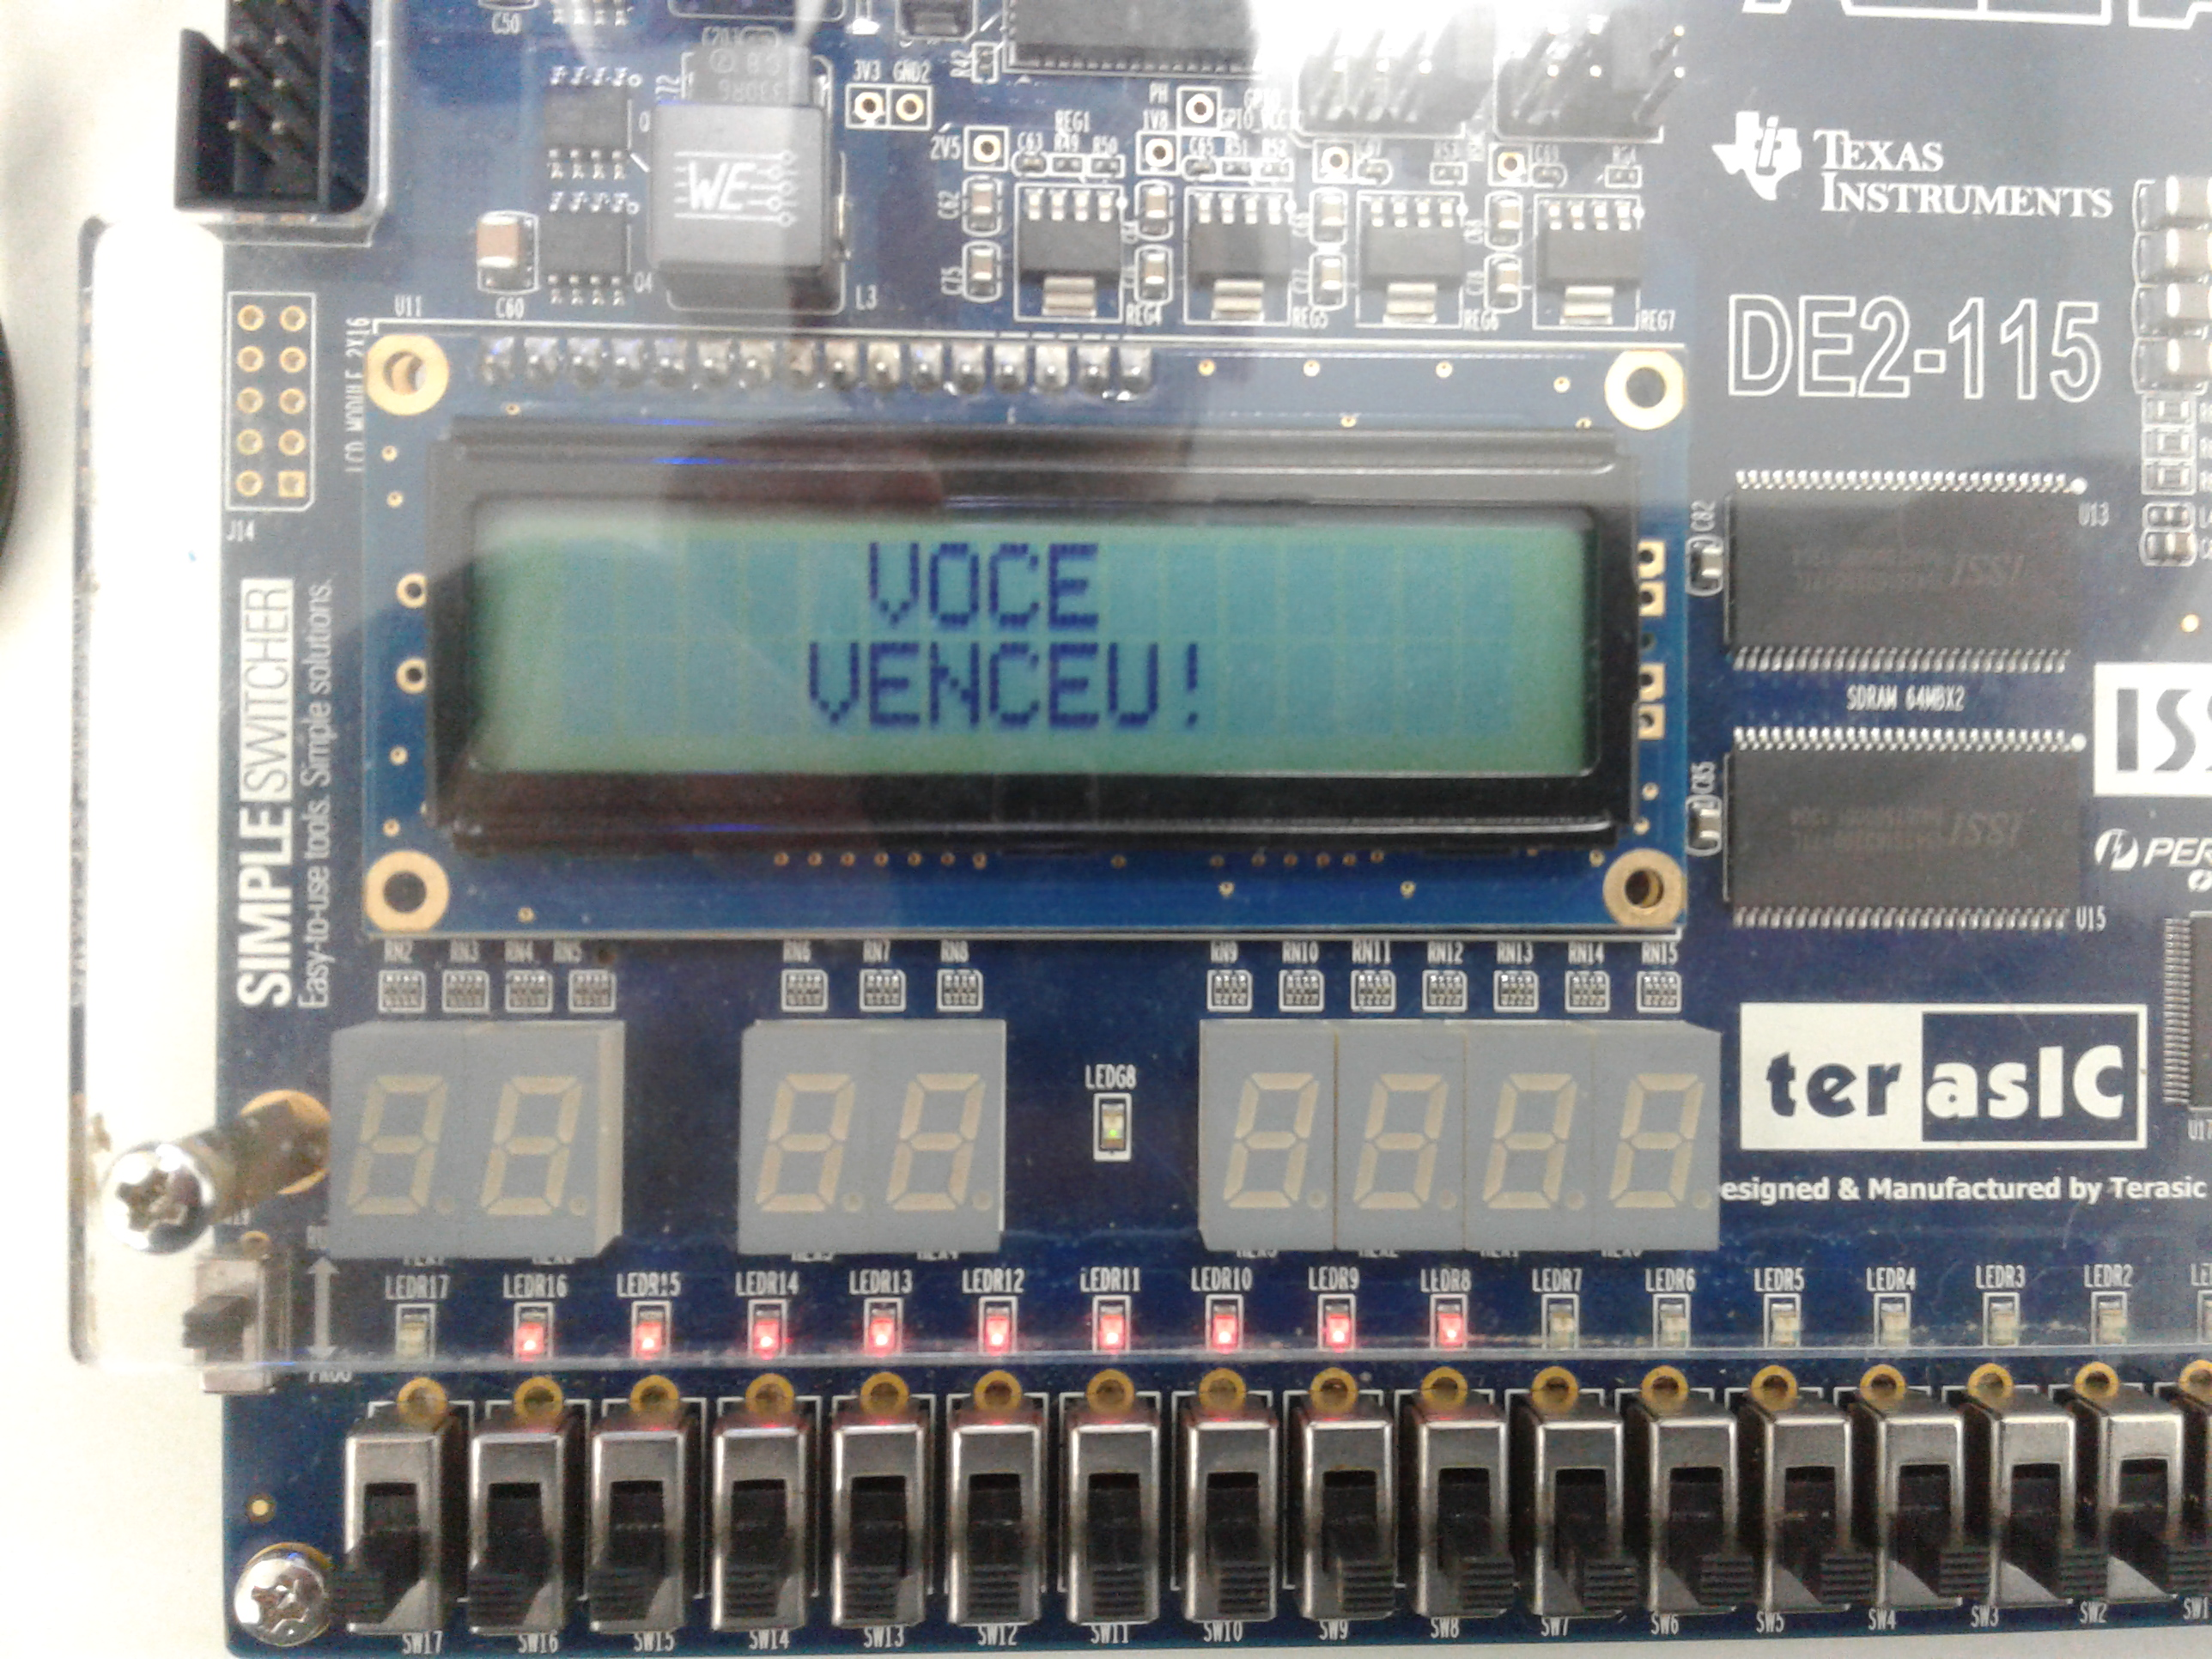
\includegraphics[scale=0.14]{foto_placa_vocevenceu.jpg}
                    \caption{Foto da placa operando no estado $S_4$}
                    \label{voce venceu}
                \end{figure}
                
                 \begin{figure}[H]
                    \centering
                    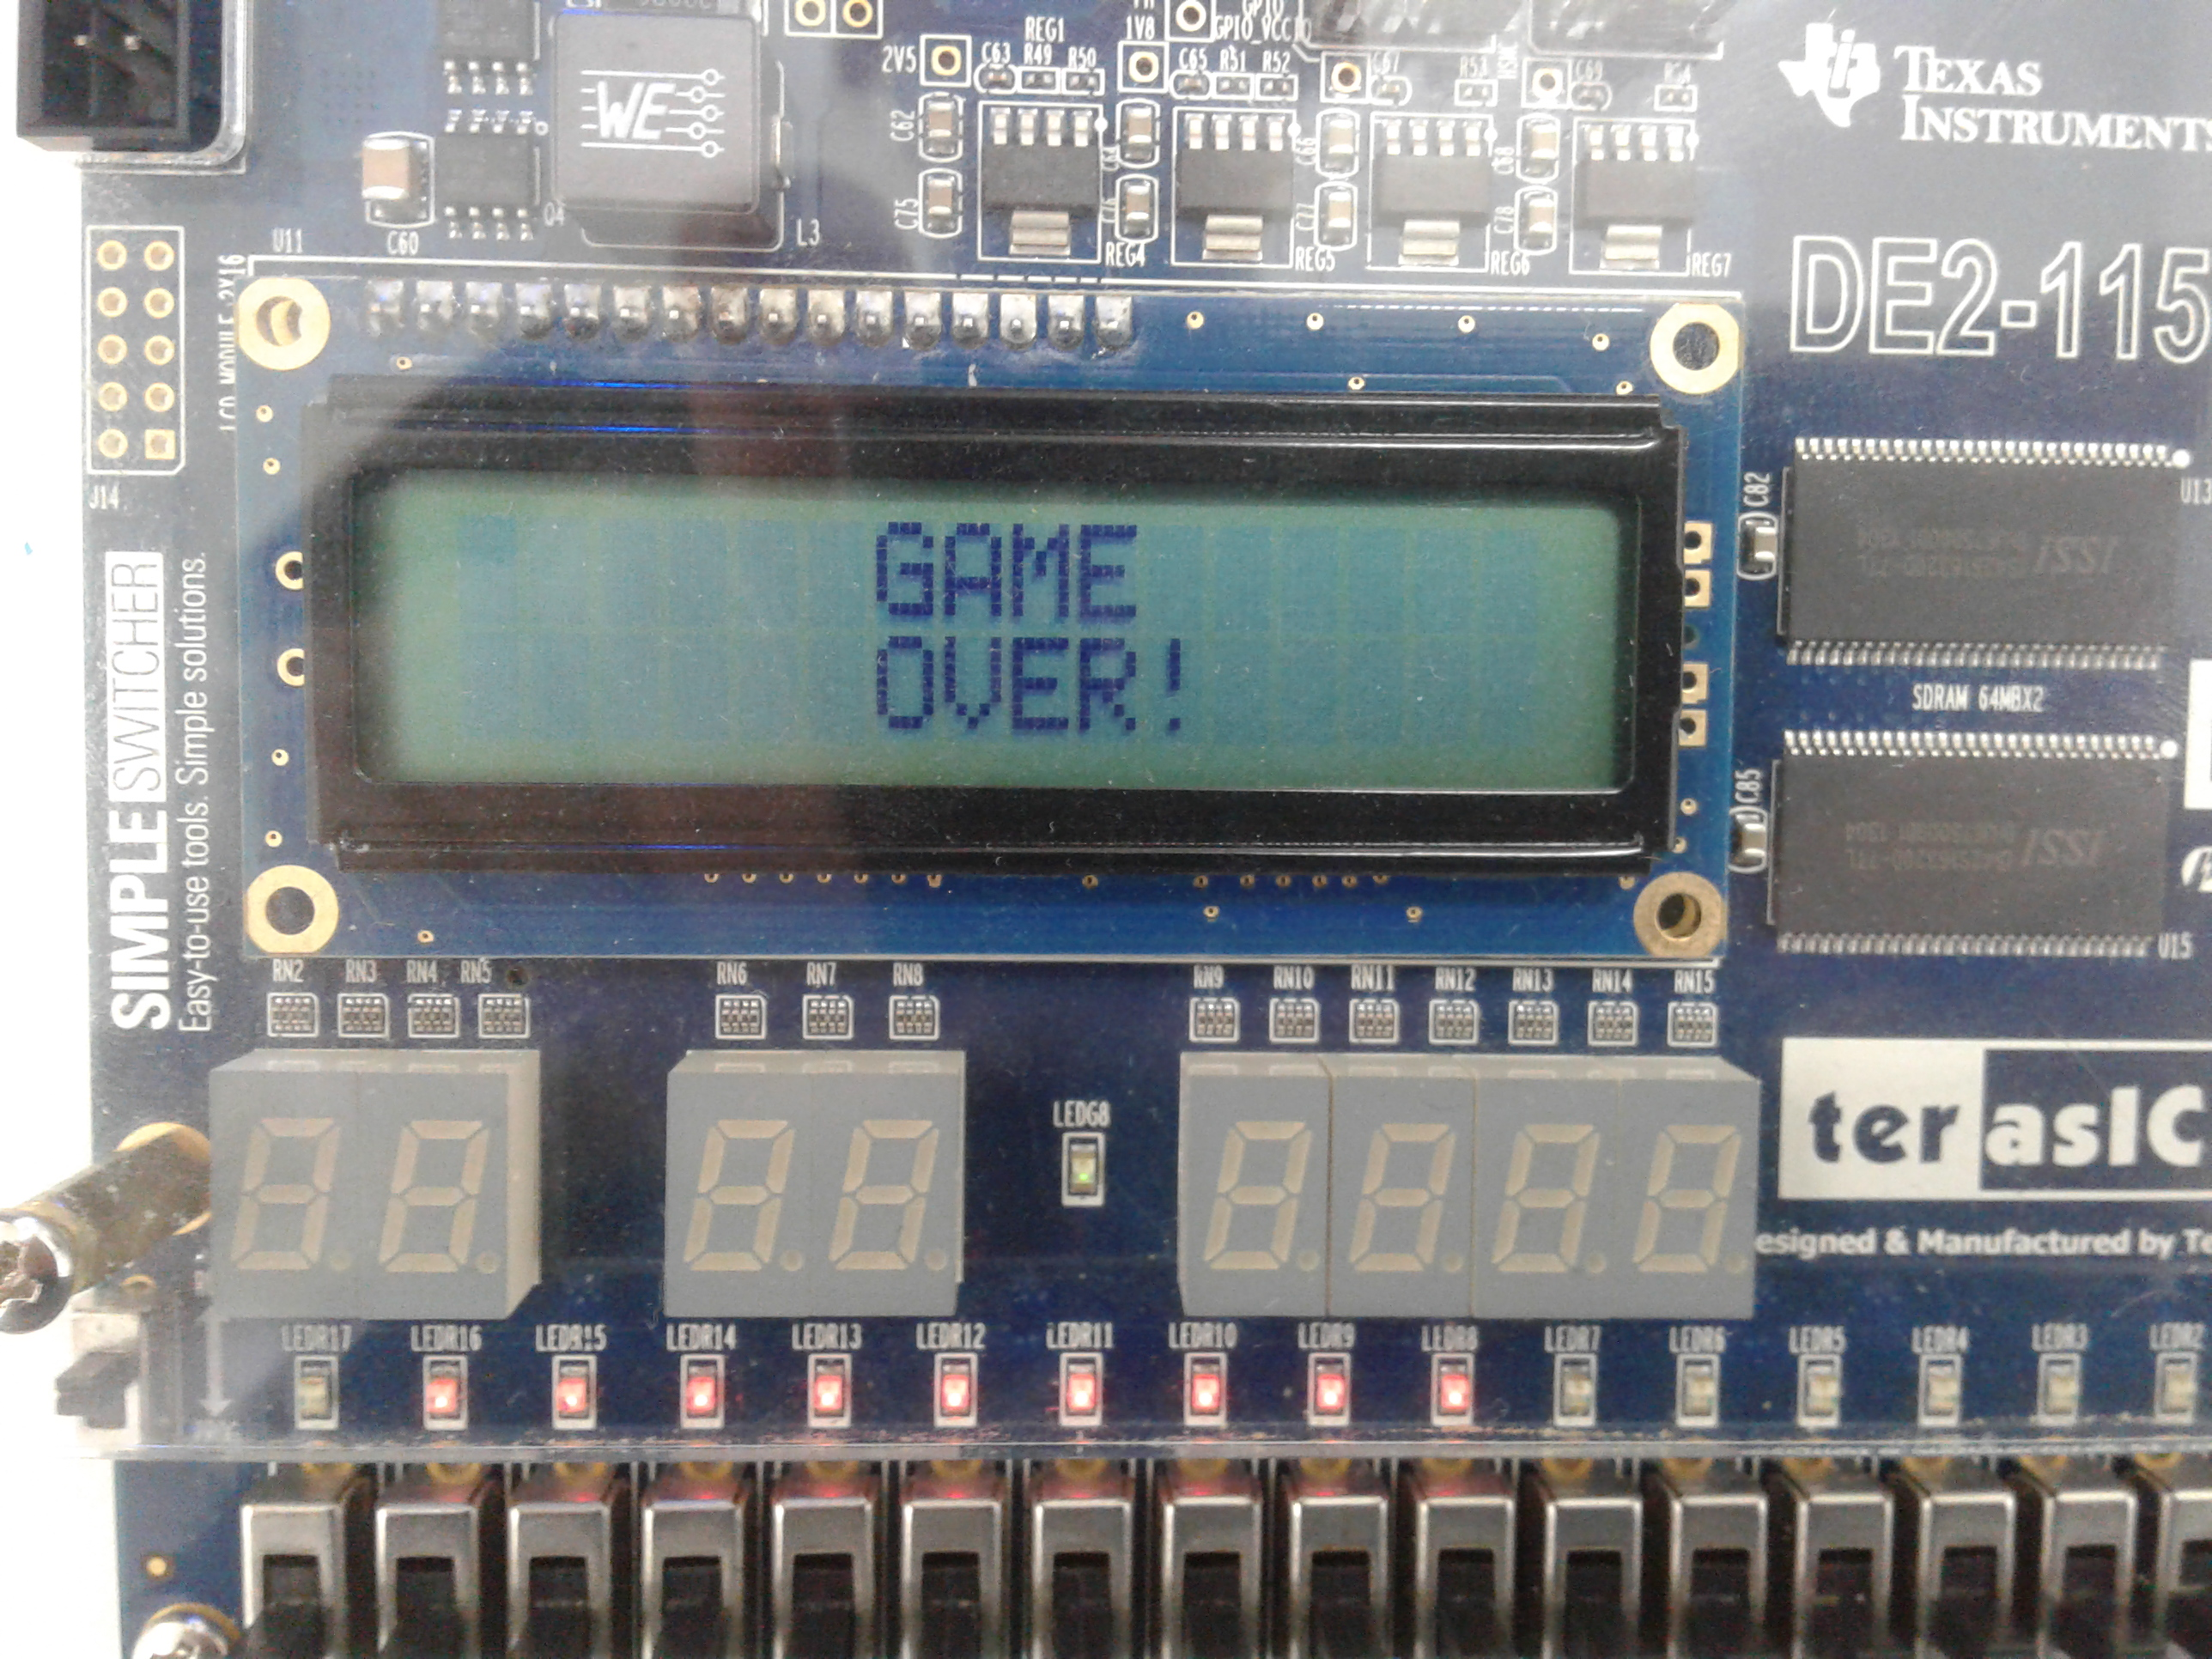
\includegraphics[scale=0.14]{foto_placa_gameover.jpg}
                    \caption{Foto da placa operando no estado $S_5$}
                    \label{game over}
                \end{figure}
                
            
        \chapter[Discussão]{\hyperlink{toc}{Discussão}} \hypertarget{ana}{}
            \tab No tocante aos problemas e dificudades encontrados no desenvolvimento do projeto cita-se a implementação do módulo infravermelho, um problema persistente comprometia a funcionalidade do circuito. Uma sobreposição de valores estava ocorrendo quando um comando era acionado repetidas vezes ou quando vários comandos eram acionados. A solução encontrada foi utilizar uma variável que verificava o término da leitura de todos os valores enviados pelo controle. Assim, somente haveria registro de uma nova sequência se a sequência anterior já houvesse sido registrada por completo ($33$ bits).
            
            \tab Menciona-se também um contratempo referente à geração da sequência aleatória. Em que, a primeira sequência gerada após a inicialização da placa era sempre a mesma e igual a "00000000". As sequências posteriores não apresentavam problemas. Para contornar esse problema, mudou-se a lógica do jogo para que fossem geradas duas sequências em estados distindo antes de sua exibição. Assim, a primeira sequência exibida não é mais a primeira seqência gerada e o problema foi consertado.
            
            \tab Finalmente, cita-se o fato de o coração não estar predefinido na tabela verdade do LCD. Sendo assim, necessário criar o coração pixel por pixel e preenchelo em um endereço vazio do CGRAM.  
                
        \chapter[Conclusão]{\hyperlink{toc}{Conclusão}}
            \tab Observa-se que o jogo de repetição funcionou bem próximo do esperado. Apesar do projeto não conseguir ser terminado completamente, é notório que as partes fundamentais do mesmo foram cumpridas com maestria. Também é digno de notar a complexidade que é trabalhar com o controle infravermelho e com o LCD, surgiram muitos bugs e dificuldades ao longo do projeto, e muitas vezes o grupo sentiu bastante dificuldade de vence-los. \\
            \tab Ao contrário do que foi argumentado nesta mesma seção no projeto anterior, desta vez, a implementação das especificações foi bem difícil, visto que o infravermelho é bastante sensível aos tempos de valor lógico alto e baixo, e o LCD deve ser manipulado de forma "fechada", ou seja, não se pode deixar variáveis soltas, isso pode acarretar em lixo de memória percorrendo ao longo da placa, fazendo com que surjam problemas como a tela ficar verde e não aparecer nenhuma mensagem. \\ 
            \tab Sendo assim, este projeto foi bastante útil para todos do grupo, além de aprender de verdade como usar VHDL, também foi possível utilizar a prática de buscar um código feito na internet, entende-lo e adaptá-lo, procedimento bastante comum, popularmente conhecido como "não reinventar a roda". 
                    
        
        
\end{document}

